% ======================================================================
% capitulos/linea2/e1_requerimientos_diseno.tex
% ----------------------------------------------------------------------
% LÍNEA CE02 — INGENIERÍA DE SOFTWARE
% S1 · E1: REQUERIMIENTOS Y DISEÑO DEL SISTEMA (alineado con CE021)
% Evidencias: CE0211, CE0212, CE0213, CE0214
% Estructura según la plantilla de la transcripción oficial (secciones 1-4 + anexos)
% ======================================================================
\chapter{Requerimientos y Diseño del Sistema}
\label{chap:ce02-e1}

\entregable{CE02 --- Ingeniería de Software · competencia CE021 Ingeniería de Requerimientos}
{Semestre 1 · Entregable 1: Requerimientos y Diseño del Sistema}
{CE0211 Especificación validada · CE0212 Prototipo navegable · CE0213 Diseño arquitectónico · CE0214 Diseño detallado}
{Completo. Pendiente: fecha y firmas del acta y enlace al prototipo publicado.}

\section*{Resumen ejecutivo}
\addcontentsline{toc}{section}{Resumen ejecutivo}

\textbf{Problema.} WISP atiende unos 455 clientes de fibra óptica en 13 zonas de Puno con
un proceso manual y disperso: la venta se anota en papel o WhatsApp, la instalación no
deja constancia de qué borne y qué equipo quedó en cada casa, los cortes se hacen a mano
en cada router y toda la administración depende de una sola persona.

\textbf{Usuarios.} Cuatro roles internos ---administrador (gerente/ingeniero), técnico,
vendedor de campo y atención al cliente--- y el cliente final, que consulta su cuenta en la
app y recibe avisos por WhatsApp.

\textbf{Alcance.} 56 requerimientos funcionales en 14 módulos (venta, aprobación,
instalación, planta externa, inventario, cobranza, cortes, comunicación, autoservicio y
operación de campo), 12 atributos de calidad y 12 reglas de negocio. Cada requerimiento
indica si ya está implementado en el producto (41), parcialmente (5) o pendiente (10).

\textbf{Solución.} Un monolito modular con API REST (FastAPI) y base PostgreSQL, un panel
web en React para la oficina y una app móvil en Expo para campo, un servicio propio de
WhatsApp y la gestión de los 13 MikroTik por SSH a través de una VPN WireGuard. Se
documenta con las vistas C4 de contexto, contenedores y componentes, nueve decisiones
arquitectónicas (ADR), diagramas UML de casos de uso, clases, secuencia y estados, y una
matriz de trazabilidad requerimiento $\rightarrow$ historia $\rightarrow$ componente
$\rightarrow$ diseño.

% ======================================================================
% capitulos/linea2/capitulo6.tex
% ----------------------------------------------------------------------
% LÍNEA CE02 — INGENIERÍA DE SOFTWARE
% Evidencia CE0211: Especificación de requerimientos validada
% Fuente: WISP_Entregable1_Linea3.docx + verificación contra el código real
%         (repositorio Wisp, rama main, 18/11/2026)
% ======================================================================
\section{Sección 1: Especificación de Requerimientos}
\label{chap:ce02-requerimientos}

Esta sección corresponde a la
evidencia \textbf{CE0211 — Especificación de requerimientos validada}. Define qué
debe hacer el \textbf{Sistema de Gestión Integral para ISP de Fibra Óptica
Multi-Zona} (en adelante, \emph{el sistema}) a partir del modelado de procesos TO-BE
(\cref{chap:procesos}) y de la solución TIC (\cref{chap:soluciontic}) de la línea
CE01.

\begin{upeubox}{Fundamento metodológico}
La especificación sigue la estructura de la norma ISO/IEC/IEEE~29148:2018
(\emph{Requirements engineering}): requerimientos funcionales agrupados por módulo,
atributos de calidad (no funcionales), reglas de negocio, restricciones e historias
de usuario con criterios de aceptación verificables. Cada requerimiento tiene un
identificador único que se rastrea hasta la arquitectura, el diseño y la base de
datos (\cref{sec:ce02-trazabilidad}).
\end{upeubox}

\begin{upeubox}{Especificación contrastada con el producto real}
A diferencia de un SRS escrito solo en papel, esta versión se \textbf{contrastó con el
código fuente} del repositorio del sistema (rama \texttt{main} al 18/11/2026). Cada
requerimiento indica su estado: \textbf{Impl.} (implementado, con evidencia en el
código), \textbf{Parcial} (implementado en parte o de otra forma) o
\textbf{Pend.} (pendiente, planificado para el semestre~2). Así el documento no
declara como hecho algo que el producto todavía no hace.
\end{upeubox}

% ======================================================================
\subsection{Contexto, problema y usuarios}
\label{sec:ce02-contexto}

WISP es un proveedor de internet por fibra óptica con sede en Juliaca (Puno) que
atiende a sus clientes en 13 zonas rurales y periurbanas, cada una con su propio
router MikroTik RB4011 y una OLT GPON. Antes del sistema, el proceso completo
—captación, instalación, inventario de equipos, cobranza, cortes y comunicación con
el cliente— se gestionaba de forma manual y dispersa (cuadernos, hojas de cálculo,
grupos de WhatsApp y acceso directo a cada router). Esto provocaba errores de
coordinación entre ventas y técnicos, pérdida de trazabilidad de qué borne y qué
equipo quedó en cada domicilio, retrasos en la cobranza y cortes inconsistentes.

\begin{table}[htbp]
\centering
\caption{Usuarios del sistema (roles reales implementados).}
\label{tab:ce02-roles}
\small
\begin{tabularx}{\textwidth}{L{3.2cm}L{3cm}X}
\toprule
\textbf{Rol} & \textbf{Canal} & \textbf{Responsabilidad principal} \\
\midrule
Administrador (\texttt{admin}) & Panel web & Gerente/ingeniero: valida ventas, administra zonas, red (WireGuard, MikroTik), planes, inventario, cobranza y usuarios. \\
Técnico (\texttt{tecnico}) & App móvil & Instala en campo (caja NAP, borne, ONU, fotos), atiende averías y retiros, administra su inventario asignado. \\
Vendedor de campo (\texttt{vendedor\_campo}) & App móvil & Capta clientes (datos, GPS, fotos) y registra su jornada y recorrido. \\
Atención al cliente (\texttt{atencion\_cliente}) & Panel web & Caja y mostrador: registra pagos, emite recibos y consulta clientes. \\
Cliente final & App móvil (PIN) y WhatsApp & Consulta su cuenta y pagos; recibe avisos de cobro y corte. \\
\bottomrule
\end{tabularx}
\end{table}

\noindent\textit{Nota de evolución:} el borrador inicial consideraba tres roles
internos (Gerente/Ingeniero, Vendedora, Técnico). Durante la validación se separó el
personal de caja como \emph{Atención al cliente} y se renombró la vendedora como
\emph{Vendedor de campo}; el modelo final tiene exactamente cuatro roles internos
(\texttt{RolUsuario} en \texttt{backend/app/models.py}).

% ======================================================================
\subsection{Requerimientos funcionales}
\label{sec:ce02-rf}

Los requerimientos se agrupan por módulo siguiendo el flujo del negocio: información
pública, venta y validación, instalación en campo, inventario, cobranza, cortes y
comunicación con el cliente.

{\small
\begin{longtable}{L{1.3cm}L{9.6cm}C{1.4cm}}
\caption{Requerimientos funcionales y su estado de implementación.}
\label{tab:ce02-rf}\\
\toprule
\textbf{Código} & \textbf{Descripción} & \textbf{Estado} \\
\midrule
\endfirsthead
\toprule
\textbf{Código} & \textbf{Descripción} & \textbf{Estado} \\
\midrule
\endhead
\midrule \multicolumn{3}{r}{\textit{Continúa en la página siguiente}} \\
\endfoot
\bottomrule
\endlastfoot
\multicolumn{3}{l}{\textbf{A. Portal web público}} \\
RF-01 & Mostrar sin autenticación las zonas con cobertura del servicio. & Impl. \\
RF-02 & Mostrar sin autenticación los planes disponibles (velocidad y precio). & Impl. \\
\multicolumn{3}{l}{\textbf{B. Usuarios y roles}} \\
RF-03 & Inicio de sesión diferenciado para los cuatro roles internos y para el cliente (PIN en la app). & Impl. \\
RF-04 & Restringir cada módulo según el rol autenticado (RBAC). & Impl. \\
\multicolumn{3}{l}{\textbf{C. Registro de ventas (vendedor de campo)}} \\
RF-05 & Registrar DNI/RUC, nombres, teléfono y WhatsApp del cliente, con autocompletado del nombre por consulta de DNI/RUC. & Impl. \\
RF-06 & Capturar automáticamente las coordenadas GPS de la vivienda. & Impl. \\
RF-07 & Adjuntar una o más fotografías de la fachada. & Impl. \\
RF-08 & Registrar dos o más fechas posibles propuestas para la visita técnica. & Pend. \\
\multicolumn{3}{l}{\textbf{D. Validación de ventas (administrador)}} \\
RF-09 & Listar las solicitudes pendientes de aprobación. & Impl. \\
RF-10 & Aprobar o rechazar una solicitud registrando el motivo del rechazo. & Impl. \\
RF-11 & Al aprobar, publicar la orden en el panel del técnico asignado a la zona del cliente. & Impl. \\
\multicolumn{3}{l}{\textbf{E. Coordinación de la visita (técnico)}} \\
RF-12 & El técnico ve únicamente las órdenes aprobadas de sus zonas asignadas. & Impl. \\
RF-13 & Enviar desde el sistema una plantilla de WhatsApp para coordinar la fecha de instalación. & Pend. \\
RF-14 & Registrar la fecha finalmente acordada con el cliente. & Pend. \\
\multicolumn{3}{l}{\textbf{F. Registro de planta externa (técnico)}} \\
RF-15 & Registrar la caja NAP y el borne utilizados en la instalación (la mufa y la corrida de origen se registran en el mapa de red). & Parcial \\
RF-16 & Validar que el borne esté libre antes de asignarlo. & Impl. \\
RF-17 & Vincular automáticamente el borne con el cliente. & Impl. \\
RF-18 & Mostrar el mapa de ocupación de bornes de cada caja (libre / ocupado / dañado). & Impl. \\
\multicolumn{3}{l}{\textbf{G. Registro del equipo instalado (técnico)}} \\
RF-19 & Seleccionar la ONU desde el inventario asignado al técnico. & Impl. \\
RF-20 & Registrar marca y estándar WiFi (WiFi~5 / WiFi~6) del equipo. & Impl. \\
RF-21 & Registrar número de serie y MAC, de forma manual o escaneando el código con la cámara. & Impl. \\
RF-22 & Adjuntar fotografías de evidencia de la instalación. & Impl. \\
RF-23 & Al cerrar la instalación, pasar la ONU a estado \emph{instalado} y descontarla del inventario del técnico. & Impl. \\
\multicolumn{3}{l}{\textbf{H. Inventario de equipos (administrador)}} \\
RF-24 & Registrar nuevas ONU escaneando su código (serie y MAC). & Impl. \\
RF-25 & Asignar ONU a un técnico específico. & Impl. \\
RF-26 & Consultar el stock por técnico y por estado (almacén, asignado, instalado, dañado, perdido). & Impl. \\
RF-27 & Reportar una ONU como dañada indicando el motivo. & Parcial \\
RF-28 & Al reportarse un equipo dañado, notificar al administrador. & Pend. \\
\multicolumn{3}{l}{\textbf{I. Pagos y facturación}} \\
RF-29 & Registrar pagos (efectivo, Yape, transferencia), incluidos adelantos de varios meses con descuento. & Impl. \\
RF-30 & Listar clientes con pagos vencidos o próximos a vencer. & Impl. \\
RF-31 & Generar automáticamente un recibo en PDF por cada cobro. & Impl. \\
RF-32 & Impedir dos pagos con el mismo número de operación. & Impl. \\
\multicolumn{3}{l}{\textbf{J. Cortes de servicio}} \\
RF-33 & Cortar manualmente el servicio de un cliente desde el sistema (address-list en el MikroTik de la zona). & Impl. \\
RF-34 & Ejecutar cortes automáticos diarios para clientes vencidos, respetando días de gracia y compromisos de pago. & Impl. \\
RF-35 & Reactivar automáticamente el servicio al registrar el pago. & Impl. \\
\multicolumn{3}{l}{\textbf{K. Notificaciones por WhatsApp}} \\
RF-36 & Enviar un mensaje de bienvenida al cerrar la instalación (plan, precio, fecha de pago). & Pend. \\
RF-37 & Enviar recordatorios automáticos de pago antes del vencimiento. & Impl. \\
RF-38 & Avisar al cliente antes de ejecutar el corte por falta de pago. & Impl. \\
\multicolumn{3}{l}{\textbf{L. Bot de WhatsApp con IA — validación de pagos}} \\
RF-39 & Recibir la fotografía de un comprobante (Yape/transferencia) enviada por el cliente. & Pend. \\
RF-40 & Solicitar DNI o nombre para ubicar al cliente. & Pend. \\
RF-41 & Extraer con IA (OCR/visión) monto, fecha y número de operación. & Pend. \\
RF-42 & Validar que el comprobante no esté registrado (duplicados). & Pend. \\
RF-43 & Confirmar el pago y enviar el recibo automáticamente. & Pend. \\
\multicolumn{3}{l}{\textbf{M. Autoservicio del cliente}} \\
RF-44 & Consultar la fecha del próximo pago. & Parcial \\
RF-45 & Consultar si tiene cuotas vencidas. & Parcial \\
RF-46 & Consultar el historial de pagos y recibos. & Parcial \\
\multicolumn{3}{l}{\textbf{N. Requerimientos incorporados durante la validación}} \\
RF-47 & Registrar averías (motivo, caja, borne, potencia óptica), asignarlas a un técnico y cerrarlas con diagnóstico y fotos. & Impl. \\
RF-48 & Gestionar órdenes de retiro de equipos (ONU, roseta, patchcord). & Impl. \\
RF-49 & Registrar la jornada del vendedor de campo (inicio/fin, recorrido GPS, pasaje y reintegros). & Impl. \\
RF-50 & Enviar mensajes masivos de WhatsApp por zona y estado, con registro por destinatario. & Impl. \\
RF-51 & Registrar gastos operativos por zona y mostrar ingresos frente a gastos. & Impl. \\
RF-52 & Gestionar clientes satelitales (Starlink) sin zona ni MikroTik. & Impl. \\
RF-53 & Administrar el túnel WireGuard de cada zona (alta/baja de peers, estado del enlace) y una terminal RouterOS restringida. & Impl. \\
RF-54 & Dibujar mufas, corridas de fibra y cajas NAP sobre el mapa de cada zona. & Impl. \\
RF-55 & Sincronizar los planes como perfiles PPPoE en los MikroTik de todas las zonas. & Impl. \\
RF-56 & Mostrar el estado de la sesión PPPoE de un cliente en tiempo real. & Impl. \\
\end{longtable}
}

\noindent Resumen: de 56 requerimientos funcionales, \textbf{41 están implementados},
\textbf{5 parcialmente} y \textbf{10 pendientes}. Los requerimientos RF-44 a RF-46 se
resolvieron mediante la \emph{App del cliente} (consulta de cuenta y pagos con PIN) en
lugar del bot conversacional; el bot con IA (RF-39 a RF-43) se reprograma para el
semestre~2 (ver ADR-06 en el \cref{chap:ce02-arquitectura}).

% ======================================================================
\subsection{Requerimientos no funcionales}
\label{sec:ce02-rnf}

Los requerimientos no funcionales describen \emph{cómo} debe comportarse el sistema, más
allá de lo que hace. Se organizan según las características de calidad de la norma
ISO/IEC~25010 (seguridad, fiabilidad, eficiencia, usabilidad, mantenibilidad y
portabilidad) y se priorizaron a partir de las condiciones reales de WISP: el sistema
maneja datos personales y dinero, por lo que la seguridad y la trazabilidad pesan más; el
técnico trabaja en zonas rurales con señal intermitente, por lo que la usabilidad en el
celular es crítica; y una MYPE con un solo administrador necesita que el sistema se
recupere y se mantenga sin depender de una sola persona.

Cada requerimiento indica cómo se verifica, para que pueda comprobarse con una prueba y no
quede como una intención. La verificación de RNF-10 (recuperación) ya se ejecutó en
laboratorio en el entregable de plataforma de datos (\cref{chap:ce02-datos}).

\begin{table}[H]
\centering
\caption{Requerimientos no funcionales (atributos de calidad ISO/IEC~25010).}
\label{tab:ce02-rnf}
\small
\begin{tabularx}{\textwidth}{L{1.4cm}L{2.3cm}XL{3.3cm}}
\toprule
\textbf{Código} & \textbf{Atributo} & \textbf{Requerimiento} & \textbf{Cómo se verifica} \\
\midrule
RNF-01 & Seguridad & Autenticación con JWT y control de acceso por rol en cada endpoint. & Pruebas de API con roles distintos. \\
RNF-02 & Seguridad & Contraseñas con bcrypt; comunicaciones solo por HTTPS/TLS; freno a la fuerza bruta en el login (8 intentos en 5 min, bloqueo de 15 min). & Revisión de configuración y prueba de bloqueo. \\
RNF-03 & Privacidad & Tratamiento de DNI, ubicación y fotos conforme a la Ley N.\textsuperscript{o}~29733; el token de consulta de DNI vive solo en el servidor. & Auditoría de datos personales. \\
RNF-04 & Disponibilidad & Recordatorios y cortes automáticos operan a diario (08:00 y 09:00, hora de Lima) sin intervención humana. & Registro del planificador. \\
RNF-05 & Usabilidad & La app del técnico funciona en smartphones de gama media y con conectividad intermitente. & Prueba en campo. \\
RNF-06 & Rendimiento & Consultas de borne y estado del cliente en menos de 2~s; el estado de WireGuard se guarda en caché 120~s para no saturar la VPS. & Medición de tiempos de respuesta. \\
RNF-07 & Confiabilidad & Ante duda en un comprobante, el caso pasa a revisión humana (aplica al bot del semestre~2). & Caso de prueba de baja confianza. \\
RNF-08 & Trazabilidad & Todo cambio relevante (activación, corte, pago, cambio de plan u ONU) queda en el historial con usuario y fecha. & Consulta de la tabla \texttt{historial}. \\
RNF-09 & Escalabilidad & Agregar zonas y clientes sin rediseño (zona = registro + peer WireGuard). & Alta de una zona de prueba. \\
RNF-10 & Recuperación & Respaldo diario de la base de datos con retención de 30 días y copia fuera del servidor. & Prueba de restauración. \\
RNF-11 & Mantenibilidad & Backend modular por dominio (19 routers) y esquema versionado con migraciones Alembic. & Revisión de código. \\
RNF-12 & Portabilidad & Todo el sistema se despliega con Docker Compose en cualquier servidor Linux. & Despliegue en un equipo limpio. \\
\bottomrule
\end{tabularx}
\end{table}

% ======================================================================
\subsection{Reglas de negocio}
\label{sec:ce02-rn}

Las reglas de negocio son las condiciones propias de la operación de WISP que el sistema
debe hacer cumplir siempre, sin importar qué usuario opera la pantalla. Se obtuvieron del
modelado de procesos TO-BE (\cref{chap:procesos}) y de la validación con el personal; por
ejemplo, que un borne no puede tener dos clientes, que un técnico solo instala equipos de
su propio inventario o que el aviso de corte se envía \emph{antes} de cortar, para que el
cliente lo reciba mientras todavía tiene internet.

La tabla indica, para cada regla, dónde se garantiza. Las que protegen la integridad de los
datos se refuerzan en la propia base de datos ---restricciones \texttt{UNIQUE}, triggers e
índices probados en el entregable de plataforma de datos---, para que se cumplan aunque una
pantalla tenga un error; las demás las aplica el backend según el rol y el estado del
cliente.

\begin{table}[H]
\centering
\caption{Reglas de negocio y dónde se hacen cumplir.}
\label{tab:ce02-reglas}
\small
\begin{tabularx}{\textwidth}{L{1.2cm}XL{3.4cm}}
\toprule
\textbf{Código} & \textbf{Regla} & \textbf{Dónde se garantiza} \\
\midrule
RN-01 & Un borne de una caja NAP no puede estar asignado a más de un cliente. & Aplicación + base de datos: índice \texttt{uq\_borne\_cliente} y trigger \texttt{trg\_validar\_borne} (\cref{sec:ce02-programacion}). \\
RN-02 & Un técnico solo instala equipos de su propio inventario asignado. & Aplicación. \\
RN-03 & Una instalación no se cierra sin fotos de evidencia y número de serie de la ONU, salvo clientes \emph{migrados}. & Aplicación. \\
RN-04 & Un técnico solo ve y atiende órdenes de sus zonas asignadas. & Aplicación (\texttt{tecnico\_zona}). \\
RN-05 & Una venta debe ser aprobada por el administrador antes de llegar a un técnico. & Aplicación (estado del cliente). \\
RN-06 & No pueden existir dos pagos con el mismo número de operación. & Base de datos (\texttt{UNIQUE}). \\
RN-07 & El corte automático se ejecuta solo si se superan los días de gracia configurados y no hay compromiso de pago vigente. & Planificador. \\
RN-08 & Al registrar el pago de un cliente cortado, el servicio se reactiva automáticamente. & Aplicación + MikroTik; en BD, procedimiento \texttt{sp\_registrar\_pago}. \\
RN-09 & El aviso de corte por WhatsApp se envía \emph{antes} de cortar, para que el cliente lo reciba con internet. & Aplicación. \\
RN-10 & La marca de cliente \emph{migrado} solo la pone quien registra desde el panel, nunca el técnico desde la app. & Aplicación. \\
RN-11 & El usuario y la contraseña PPPoE salen siempre del DNI (nunca del RUC, que es público). & Aplicación. \\
RN-12 & Solo el administrador ve la configuración de red (túnel, router, IP) y ejecuta cortes manuales. & Aplicación (RBAC). \\
\bottomrule
\end{tabularx}
\end{table}

% ======================================================================
\subsection{Restricciones del sistema}
\label{sec:ce02-restricciones}

\begin{itemize}
  \item \textbf{Presupuesto de MYPE:} se prioriza una arquitectura simple y de bajo
  costo operativo (un servidor en la oficina y una VPS pequeña) frente a soluciones
  de alta complejidad.
  \item \textbf{Conectividad de campo:} los técnicos trabajan en zonas rurales con
  cobertura móvil intermitente.
  \item \textbf{Infraestructura heredada:} cada zona ya opera con un MikroTik y
  convenciones propias (nombres de pool PPPoE y de la lista de corte distintos por
  zona); el sistema debe adaptarse sin reconfigurar la red de golpe.
  \item \textbf{Sin IP pública en la oficina:} el sistema se publica mediante un túnel
  de salida (Cloudflare Tunnel) y la red se gestiona a través de una VPS con WireGuard.
  \item \textbf{Marco legal:} Ley N.\textsuperscript{o}~29733 de Protección de Datos
  Personales y su reglamento.
  \item \textbf{Mensajería:} la integración de WhatsApp depende de una sesión
  vinculada y de las políticas de la plataforma (riesgo de bloqueo por envíos masivos).
\end{itemize}

% ======================================================================
\subsection{Historias de usuario y criterios de aceptación}
\label{sec:ce02-hu}

Las historias siguen el formato \emph{Como [rol], quiero [acción], para [beneficio]}
con criterios de aceptación verificables (enfoque \emph{Given/When/Then} resumido).

\newcommand{\historia}[4]{%
\begin{tcolorbox}[enhanced,breakable,colback=white,colframe=upeublue!60,
  boxrule=0.5pt,arc=1pt,left=6pt,right=6pt,top=4pt,bottom=4pt,
  title={\small\textbf{#1} --- #2},coltitle=upeublue,colbacktitle=upeublue!8]
\small #3

\smallskip\textbf{Criterios de aceptación:}
\begin{itemize}[leftmargin=1.2em,itemsep=0pt]
#4
\end{itemize}
\end{tcolorbox}}

\historia{HU-01}{Vendedor de campo · RF-05 a RF-07}
{Como vendedor de campo, quiero registrar los datos, la ubicación y las fotos de un
cliente potencial, para iniciar su contratación sin papeles.}
{\item DNI/RUC, nombre y teléfono son obligatorios; al escribir el DNI el nombre se autocompleta.
 \item Las coordenadas se toman del GPS del dispositivo, no se escriben a mano.
 \item Se adjunta al menos una foto de la fachada.
 \item Al guardar, el cliente queda en estado \texttt{pendiente\_aprobacion}.}

\historia{HU-02}{Administrador · RF-09 a RF-11}
{Como administrador, quiero aprobar o rechazar las ventas registradas, para asegurar
que los datos son correctos antes de enviar un técnico.}
{\item El panel lista los clientes en \texttt{pendiente\_aprobacion}.
 \item Aprobar cambia el estado a \texttt{aprobado}; rechazar exige un motivo.
 \item Al aprobar, la orden aparece en la app del técnico asignado a esa zona.}

\historia{HU-03}{Técnico · RF-12}
{Como técnico, quiero ver solo las instalaciones de mis zonas, para saber qué me
corresponde sin depender de mensajes externos.}
{\item El listado filtra por las zonas asignadas en \texttt{tecnico\_zona}.
 \item Cada orden muestra los datos cargados por el vendedor y su ubicación en el mapa.}

\historia{HU-04}{Técnico · RF-15 a RF-18}
{Como técnico, quiero registrar la caja NAP y el borne que uso, para dejar constancia
exacta de la conexión física del cliente.}
{\item El sistema muestra los bornes de la caja diferenciando libres, ocupados y dañados.
 \item No se puede elegir un borne ocupado.
 \item Al confirmar, el borne queda vinculado al cliente y en estado \texttt{ocupado}.}

\historia{HU-05}{Técnico · RF-19 a RF-23}
{Como técnico, quiero registrar la ONU que dejo instalada desde mi inventario, para que
el sistema controle el stock y la trazabilidad por número de serie.}
{\item Solo aparecen ONU con estado \texttt{asignado\_tecnico} a ese técnico.
 \item La serie/MAC se puede escanear con la cámara.
 \item Al cerrar la instalación, la ONU pasa a \texttt{instalado} y el cliente a \texttt{activo}.}

\historia{HU-06}{Técnico · RF-47}
{Como técnico, quiero atender averías con diagnóstico, potencia óptica y fotos, para
resolverlas y dejar evidencia del trabajo.}
{\item La avería pasa por \texttt{pendiente} $\rightarrow$ \texttt{asignada} $\rightarrow$ \texttt{en\_proceso} $\rightarrow$ \texttt{resuelta}.
 \item Si se reemplaza la ONU, se registran la retirada y la nueva.}

\historia{HU-07}{Administrador · RF-24 a RF-26}
{Como administrador, quiero registrar y asignar ONU escaneando su código, para
controlar el inventario sin digitar cada número de serie.}
{\item Al escanear, el sistema completa la serie y permite corregirla si la lectura falla.
 \item El stock se consulta por técnico y por estado.}

\historia{HU-08}{Atención al cliente · RF-29 a RF-32}
{Como personal de atención, quiero registrar pagos y emitir el recibo, para cobrar en
mostrador de forma rápida y sin errores.}
{\item Se puede registrar un adelanto de varios meses con un solo recibo.
 \item Un número de operación repetido se rechaza.
 \item Si el cliente estaba cortado, el servicio se reactiva al registrar el pago.}

\historia{HU-09}{Administrador · RF-33 a RF-35}
{Como administrador, quiero que los cortes por mora sean automáticos y poder cortar
manualmente, para gestionar la cobranza sin entrar a cada router.}
{\item Cada día a las 09:00 se cortan los clientes vencidos más allá de los días de gracia.
 \item Se respetan los compromisos de pago vigentes.
 \item El corte agrega la IP del cliente a la lista de corte configurada para su zona.}

\historia{HU-10}{Cliente · RF-37, RF-38}
{Como cliente, quiero recibir avisos antes del vencimiento y antes del corte, para
pagar a tiempo y no quedarme sin servicio por olvido.}
{\item El recordatorio se envía unos días antes del vencimiento (08:00).
 \item El aviso de corte llega antes de que se ejecute el corte.}

\historia{HU-11}{Cliente · RF-44 a RF-46}
{Como cliente, quiero consultar en la app cuándo vence mi servicio y mis pagos, para
resolver mis dudas sin llamar a la empresa.}
{\item El cliente entra con su PIN.
 \item Ve su plan, el estado de su servicio, su fecha de vencimiento y el historial de pagos.}

\historia{HU-12}{Vendedor de campo · RF-49}
{Como vendedor de campo, quiero registrar mi jornada y recorrido, para que la empresa
vea mi trabajo y me reintegre el pasaje.}
{\item La jornada guarda el punto de inicio, los puntos del recorrido y el de fin.
 \item El administrador ve el recorrido en el mapa y marca el reintegro.}

% ======================================================================
\subsection{Validación con los interesados}
\label{sec:ce02-validacion}

La especificación y el prototipo (\cref{chap:ce02-prototipo}) se revisaron con los
perfiles de usuario de WISP (gerencia/ingeniería, ventas, técnico de campo y atención).
Los cambios acordados ya forman parte de este documento:

\begin{itemize}
  \item La ubicación se captura por GPS y no como texto, para evitar errores de tipeo (RF-06).
  \item El técnico pidió ver la caja NAP como un mapa visual de bornes y no como lista (RF-18).
  \item El administrador pidió que, al escanear un equipo, el dato leído se muestre
  de inmediato para corregirlo si la lectura falla (RF-24).
  \item Se agregaron los módulos de averías, retiros, jornadas, mensajes masivos,
  gastos y clientes satelitales (RF-47 a RF-52), que el negocio necesitaba y no
  estaban en el borrador.
  \item El cliente prefirió una app con su cuenta en lugar de esperar al bot; el bot
  con IA queda para una iteración posterior.
\end{itemize}

\begin{table}[htbp]
\centering
\caption{Acta de validación de requerimientos (Anexo de la evidencia CE0211).}
\label{tab:ce02-acta}
\small
\begin{tabularx}{\textwidth}{L{3.6cm}X}
\toprule
\textbf{Campo} & \textbf{Detalle} \\
\midrule
Proyecto & Sistema de Gestión Integral para ISP de Fibra Óptica Multi-Zona (WISP) \\
Objetivo de la sesión & Validar la especificación de requerimientos y el prototipo navegable. \\
Fecha y lugar & \rule{4cm}{0.4pt} \quad Oficina central de WISP, Juliaca \\
Participantes & Gerente/Ingeniero, vendedor de campo, técnico de campo, personal de atención, equipo del proyecto \\
Resultado & Requerimientos aprobados con las observaciones listadas arriba. \\
\bottomrule
\end{tabularx}

\medskip
\begin{tabularx}{\textwidth}{XXX}
\rule{4.2cm}{0.4pt} & \rule{4.2cm}{0.4pt} & \rule{4.2cm}{0.4pt} \\
Gerente / Ingeniero & Técnico de campo & Vendedor de campo \\
\end{tabularx}
\end{table}

\begin{upeubox}{Pendiente antes de la entrega}
El acta debe completarse con la fecha real de la sesión y las firmas de los
participantes. Un acta sin firmas no se considera evidencia de validación.
\end{upeubox}

% ======================================================================
\subsection{Matriz de trazabilidad de requerimientos}
\label{sec:ce02-trazabilidad}

{\small
\begin{longtable}{L{2.5cm}L{1.4cm}L{4.6cm}L{4.4cm}}
\caption{Trazabilidad requerimiento $\rightarrow$ historia $\rightarrow$ componente $\rightarrow$ diseño/datos.}
\label{tab:ce02-trazabilidad}\\
\toprule
\textbf{Requerimientos} & \textbf{HU} & \textbf{Componente (router / pantalla)} & \textbf{Diseño y datos} \\
\midrule
\endfirsthead
\toprule
\textbf{Requerimientos} & \textbf{HU} & \textbf{Componente (router / pantalla)} & \textbf{Diseño y datos} \\
\midrule
\endhead
\bottomrule
\endlastfoot
RF-01, RF-02 & --- & Sitio público (\texttt{web/}), \texttt{zonas.py} (\texttt{/publicas}) & Tablas \texttt{zonas}, \texttt{planes} \\
RF-03, RF-04 & --- & \texttt{auth.py}, \texttt{cliente\_app.py} & Tabla \texttt{usuarios}; \texttt{clientes.pin\_app} \\
RF-05 a RF-07 & HU-01 & \texttt{clientes.py}, \texttt{consultas.py}; app \texttt{(vendedor)/nuevo-cliente} & Secuencia de venta; tabla \texttt{clientes} \\
RF-09 a RF-11 & HU-02 & \texttt{clientes.py}; panel \texttt{AprobarClienteDialog} & Estados del cliente \\
RF-12 & HU-03 & \texttt{clientes.py}; app \texttt{(tecnico)/instalaciones} & Tabla \texttt{tecnico\_zona} \\
RF-15 a RF-18 & HU-04 & \texttt{cajas\_nap.py}, \texttt{mufas.py}; app \texttt{(tecnico)/instalar} & Secuencia de instalación; tablas \texttt{cajas\_nap}, \texttt{bornes} \\
RF-19 a RF-26 & HU-05, HU-07 & \texttt{onus.py}; app \texttt{escanear-equipo}, \texttt{inventario} & Estados de la ONU; tabla \texttt{onus} \\
RF-29 a RF-32 & HU-08 & \texttt{pagos.py}, \texttt{recibos.py} & Tabla \texttt{pagos} (\texttt{UNIQUE numero\_operacion}) \\
RF-33 a RF-35 & HU-09 & \texttt{clientes.py}, \texttt{scheduler.py} & Secuencia de corte; tabla \texttt{historial} \\
RF-37, RF-38, RF-50 & HU-10 & \texttt{whatsapp.py}, servicio \texttt{whatsapp/} & Tablas \texttt{mensajes\_masivos*} \\
RF-44 a RF-46 & HU-11 & \texttt{cliente\_app.py}; app \texttt{(cliente)/} & Tablas \texttt{clientes}, \texttt{pagos} \\
RF-47, RF-48 & HU-06 & \texttt{averias.py}, \texttt{ordenes\_retiro.py}, \texttt{evidencias.py} & Tablas \texttt{averias}, \texttt{ordenes\_retiro}, \texttt{evidencias} \\
RF-49 & HU-12 & \texttt{jornadas.py}; app \texttt{(vendedor)/jornada} & Tablas \texttt{jornadas\_vendedor}, \texttt{ubicaciones\_vendedor} \\
RF-51 & --- & \texttt{gastos.py}, \texttt{dashboard.py} & Tabla \texttt{gastos} \\
RF-53, RF-55, RF-56 & --- & \texttt{zonas.py}, \texttt{planes.py} & Despliegue (WireGuard); tabla \texttt{zonas} \\
\end{longtable}
}

% ======================================================================
% capitulos/linea2/capitulo7.tex
% ----------------------------------------------------------------------
% LÍNEA CE02 — Evidencia CE0212: Prototipo navegable validado
% ======================================================================
\section{Sección 2: Prototipo Navegable}
\label{chap:ce02-prototipo}

Esta sección corresponde a la evidencia \textbf{CE0212 — Prototipo navegable
validado}. El prototipo permitió validar con los usuarios la disposición de la
información y el flujo de trabajo \emph{antes} de construir el sistema definitivo, y
fue la base de las observaciones recogidas en el acta de la
\cref{sec:ce02-validacion}.

% ======================================================================
\subsection{Fidelidad y alcance}

Se construyó un prototipo interactivo de \textbf{fidelidad media} (clicable, con datos
de ejemplo) como aplicación web independiente en HTML, CSS y JavaScript, sin conexión
a un backend. Cubre las pantallas principales de los roles internos y una simulación
de la conversación del cliente por WhatsApp. Permite cambiar de rol desde el menú
lateral y recorrer el flujo real: venta $\rightarrow$ aprobación $\rightarrow$
coordinación $\rightarrow$ instalación $\rightarrow$ cobranza y corte.

\begin{table}[htbp]
\centering
\caption{Ficha del prototipo.}
\label{tab:ce02-ficha-proto}
\small
\begin{tabularx}{\textwidth}{L{3.5cm}X}
\toprule
Tipo & Prototipo de fidelidad media, navegable \\
Tecnología & HTML5, CSS3 y JavaScript (sin backend) \\
Pantallas & 10 pantallas principales + flujo de navegación \\
Roles cubiertos & Administrador (gerente/ingeniero), vendedor de campo, técnico y cliente (WhatsApp) \\
Validación & Sesión de revisión con usuarios de WISP (\cref{tab:ce02-acta}) \\
Enlace / repositorio & \rule{7cm}{0.4pt} \emph{(completar con la URL del prototipo publicado)} \\
\bottomrule
\end{tabularx}
\end{table}

% ======================================================================
\subsection{Flujo de navegación}

El diagrama resume cómo se conectan las pantallas y cómo la confirmación de una
instalación o un corte disparan la comunicación con el cliente.

\begin{figure}[htbp]
\centering
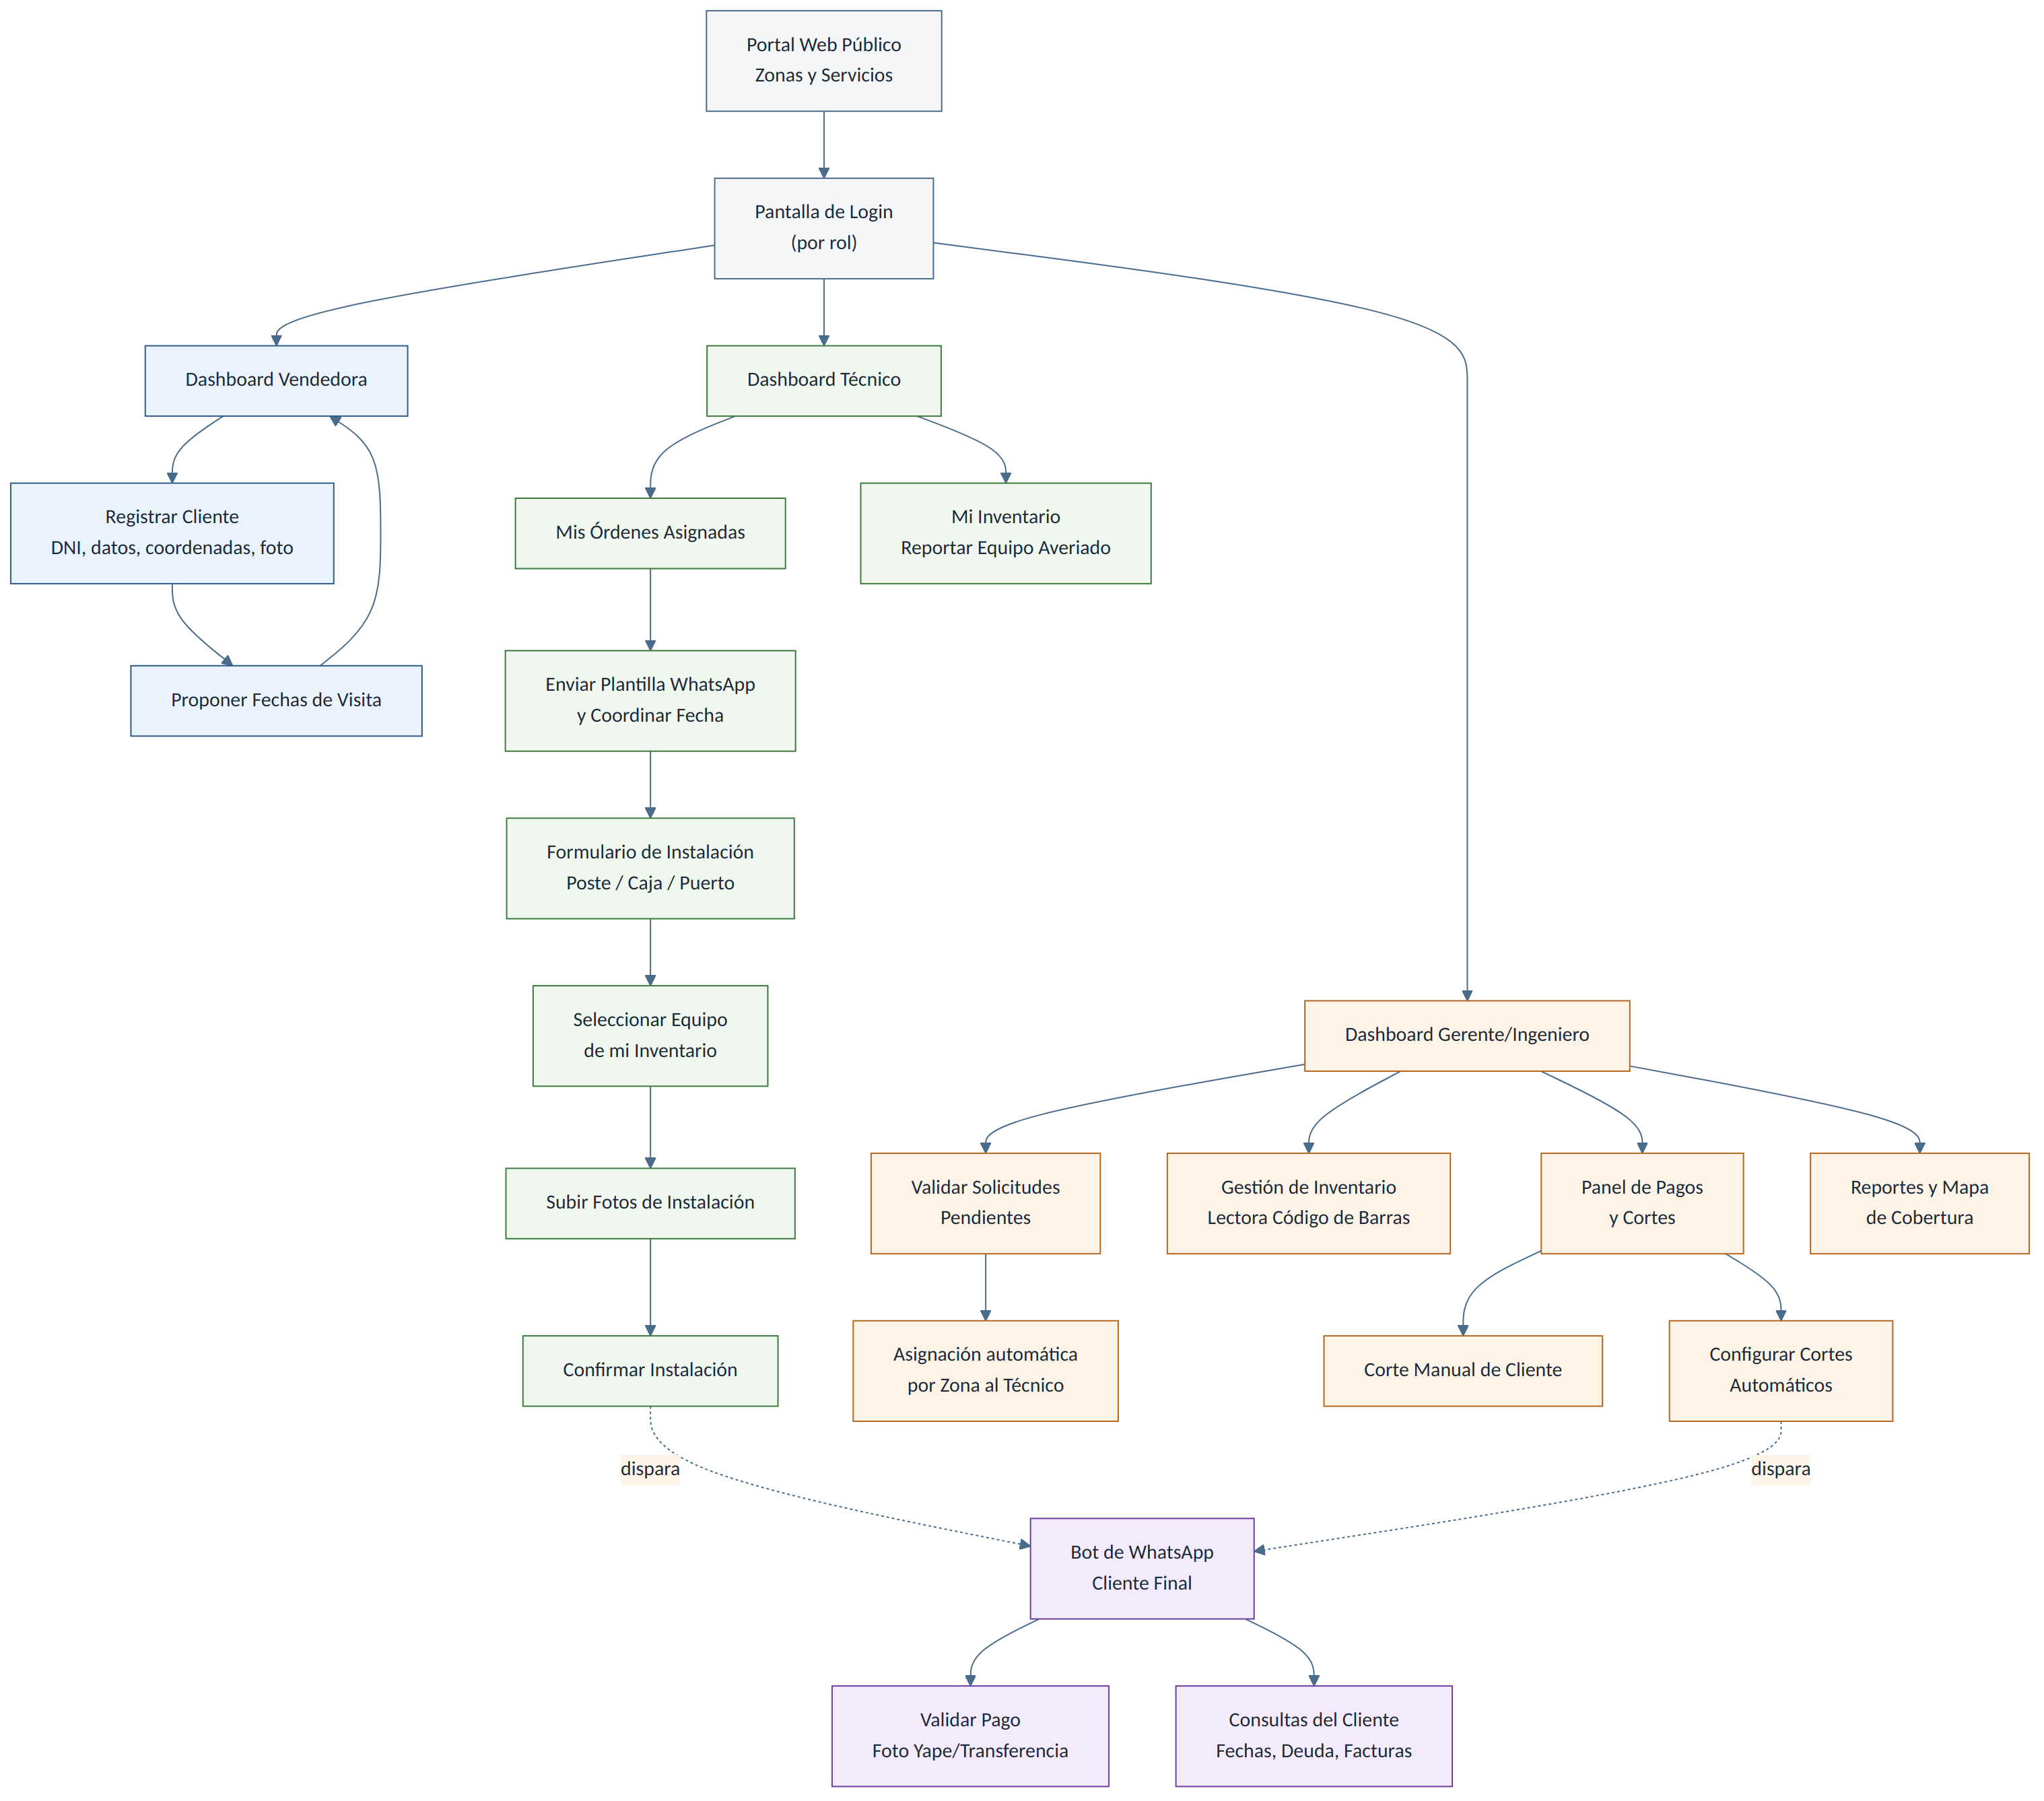
\includegraphics[width=\textwidth,height=0.42\textheight,keepaspectratio]{linea2/flujo_navegacion.png}
\caption{Flujo de navegación entre pantallas por rol.}
\label{fig:ce02-flujo}
\end{figure}

% ======================================================================
\subsection{Pantallas principales}

\newcommand{\pantalla}[3]{%
\begin{minipage}[t]{0.48\textwidth}\centering
\includegraphics[width=\linewidth,height=5.2cm,keepaspectratio]{linea2/#1}
\captionof{figure}{#2}\label{fig:ce02-#1}
\vspace{2pt}{\footnotesize\itshape #3}
\end{minipage}}

\begin{center}
\pantalla{proto_portal.png}{Portal público.}{Zonas de cobertura y planes, sin autenticación (RF-01, RF-02).}\hfill
\pantalla{proto_panel_vendedora.png}{Panel del vendedor.}{Solicitudes registradas y su estado.}
\end{center}
\begin{center}
\pantalla{proto_registro_cliente.png}{Registro de cliente.}{Datos, GPS y fotos de la vivienda (RF-05 a RF-08).}\hfill
\pantalla{proto_dashboard_tecnico.png}{Panel del técnico.}{Órdenes de su zona e inventario (RF-12).}
\end{center}
\begin{center}
\pantalla{proto_coordinar_visita.png}{Coordinar visita.}{Plantilla de WhatsApp para acordar la fecha (RF-13, RF-14).}\hfill
\pantalla{proto_registrar_instalacion.png}{Registrar instalación.}{Caja NAP, borne y equipo (RF-15 a RF-22).}
\end{center}
\begin{center}
\pantalla{proto_panel_gerencia.png}{Panel de gerencia.}{Indicadores y validación de ventas (RF-09 a RF-11).}\hfill
\pantalla{proto_inventario.png}{Inventario y lectora.}{Registro de equipos por código (RF-24 a RF-26).}
\end{center}
\begin{center}
\pantalla{proto_pagos_cortes.png}{Pagos y cortes.}{Estado de cuenta y corte manual o automático (RF-29 a RF-35).}\hfill
\pantalla{proto_bot_whatsapp.png}{Bot de WhatsApp.}{Simulación de validación de pago y consulta (RF-39 a RF-46).}
\end{center}

% ======================================================================
\subsection{Resultados de la validación}

\begin{table}[H]
\centering
\caption{Observaciones del prototipo y cómo se incorporaron al producto.}
\label{tab:ce02-obs-proto}
\small
\begin{tabularx}{\textwidth}{L{2.6cm}XL{3.8cm}}
\toprule
\textbf{Usuario} & \textbf{Observación} & \textbf{Incorporación} \\
\midrule
Vendedor & Capturar la ubicación por GPS y no escribirla. & RF-06; app móvil con \texttt{expo-location}. \\
Técnico & Ver la caja NAP como mapa visual de bornes. & RF-18; detalle de caja en la app y el panel. \\
Administrador & Mostrar de inmediato el dato escaneado para corregirlo. & RF-24; pantalla \texttt{escanear-equipo}. \\
Técnico & El técnico no debe imponer la fecha: solo la coordina con el cliente. & RF-13, RF-14 (pendientes). \\
Cliente / gerencia & Consultar la cuenta sin esperar al bot. & RF-44 a RF-46 resueltos con la App del cliente. \\
\bottomrule
\end{tabularx}
\end{table}

\begin{upeubox}{Del prototipo al producto}
El prototipo validó el flujo; el producto construido (\cref{chap:ce02-arquitectura})
lo implementa en un panel web (React) para administración y atención, y en una app
móvil (Expo) con tres espacios: técnico, vendedor y cliente. Las pantallas de
coordinación de visita y del bot con IA quedaron como trabajo pendiente del
semestre~2.
\end{upeubox}

% ======================================================================
% capitulos/linea2/capitulo8.tex
% ----------------------------------------------------------------------
% LÍNEA CE02 — Evidencia CE0213: Diseño arquitectónico del sistema
% Fuente: código real (rama main) — docker-compose.yml, backend/app, mobile/,
%         frontend/, whatsapp/, docs/DESPLIEGUE-OFICINA.md
% ======================================================================
\section{Sección 3: Diseño Arquitectónico}
\label{chap:ce02-arquitectura}

Esta sección corresponde a la evidencia \textbf{CE0213 — Diseño arquitectónico del
sistema}. Describe la estructura principal del sistema, sus componentes y
responsabilidades, su despliegue y las decisiones técnicas que lo justifican,
siguiendo el modelo C4 (contexto, contenedores y componentes) y el formato de registro
de decisiones arquitectónicas (ADR) de Michael Nygard.

% ======================================================================
\subsection{Documento de arquitectura}
\label{sec:ce02-doc-arq}

El sistema es un \textbf{monolito modular con arquitectura cliente-servidor}. Un
único backend (FastAPI), organizado internamente por dominios de negocio, expone una
API REST que consumen tres clientes: el panel web interno (React), la app móvil
(Expo/React Native) y el sitio público. El backend persiste en una base de datos
PostgreSQL, envía mensajes a través de un servicio de WhatsApp propio y gestiona los
routers MikroTik de las 13 zonas por SSH a través de una VPN WireGuard.

\begin{table}[htbp]
\centering
\caption{Atributos de calidad que guían la arquitectura.}
\label{tab:ce02-atributos}
\small
\begin{tabularx}{\textwidth}{L{2.6cm}XL{2.6cm}}
\toprule
\textbf{Atributo} & \textbf{Táctica arquitectónica aplicada} & \textbf{RNF} \\
\midrule
Seguridad & JWT + RBAC por endpoint; servicios internos atados a \texttt{127.0.0.1}; token compartido entre backend y servicio de WhatsApp; gestión de red solo por VPN. & RNF-01, 02, 03 \\
Disponibilidad & Contenedores con \texttt{restart: unless-stopped}; tareas programadas dentro del backend; límites de CPU/RAM al servicio más inestable (WhatsApp). & RNF-04 \\
Rendimiento & Caché de 120~s del estado WireGuard; pings a routers en paralelo. & RNF-06 \\
Mantenibilidad & 19 routers por dominio; esquema versionado con Alembic; configuración por variables de entorno. & RNF-11 \\
Portabilidad & Todo en Docker Compose; el mismo despliegue sirve en VPS o en la oficina cambiando una variable. & RNF-12 \\
\bottomrule
\end{tabularx}
\end{table}

% ----------------------------------------------------------------------
\subsection{Vista de contexto (C4 nivel 1)}

\begin{figure}[H]
\centering
\begin{tikzpicture}[node distance=9mm and 12mm]
  \node[caja,minimum width=4.2cm,minimum height=13mm,fill=upeublue!15,font=\small\bfseries] (sis) {Sistema de Gestión\\Integral WISP};
  \node[cajaext,above left=of sis] (adm) {Administrador /\\Atención al cliente};
  \node[cajaext,above right=of sis] (campo) {Técnico /\\Vendedor de campo};
  \node[cajaext,left=of sis] (cli) {Cliente final};
  \node[cajaext,right=of sis] (vis) {Visitante\\(público)};
  \node[cajaext,below left=of sis] (wa) {WhatsApp};
  \node[cajaext,below=of sis] (mk) {13 routers MikroTik\\(RouterOS 7)};
  \node[cajaext,below right=of sis] (api) {APIs Perú\\(DNI/RUC)};
  \draw[flecha] (adm) -- node[font=\tiny,sloped,above]{panel web} (sis);
  \draw[flecha] (campo) -- node[font=\tiny,sloped,above]{app móvil} (sis);
  \draw[flecha] (cli) -- node[font=\tiny,above]{app (PIN)} (sis);
  \draw[flecha] (vis) -- node[font=\tiny,above]{sitio web} (sis);
  \draw[flecha] (sis) -- node[font=\tiny,sloped,above]{avisos} (wa);
  \draw[flecha] (sis) -- node[font=\tiny,right]{SSH por WireGuard} (mk);
  \draw[flecha] (sis) -- node[font=\tiny,sloped,above]{consulta} (api);
\end{tikzpicture}
\caption{Vista de contexto: actores y sistemas externos.}
\label{fig:ce02-contexto}
\end{figure}

% ======================================================================
\subsection{Vista de contenedores (C4 nivel 2)}
\label{sec:ce02-componentes}

\begin{figure}[H]
\centering
\begin{tikzpicture}[x=1cm,y=1cm,scale=0.93,every node/.style={transform shape}]
  % Clientes
  \node[cajaext,minimum width=2.5cm] (nav) at (0,1.7) {Navegador\\(admin / atención)};
  \node[cajaext,minimum width=2.5cm] (app) at (0,0) {App móvil Expo\\(técnico, vendedor,\\cliente)};
  \node[cajaext,minimum width=2.5cm] (pub) at (0,-1.7) {Navegador\\(visitante)};
  % Borde
  \node[cajaext,minimum height=30mm,minimum width=1.7cm] (cf) at (2.9,0) {Cloudflare\\(HTTPS,\\túnel)};
  \node[caja,minimum height=30mm,minimum width=1.8cm] (ngx) at (5.0,0) {Nginx\\proxy\\inverso\\+ cabeceras\\de seguridad};
  % Contenedores del servidor
  \node[caja,minimum width=3.1cm] (front) at (8.2,2.3) {Panel web\\React 19 + Vite (SPA)};
  \node[caja,minimum width=3.1cm,fill=upeublue!15] (back) at (8.2,-0.3) {\textbf{API REST FastAPI}\\19 routers por dominio\\+ APScheduler};
  \node[caja,minimum width=3.1cm] (web) at (8.2,1.15) {Sitio público\\HTML/CSS/JS};
  \node[caja] (media) at (5.0,-2.8) {Volumen\\media / backups};
  \node[bd] (pg) at (7.4,-2.8) {PostgreSQL 15};
  \node[caja] (wa) at (10.0,-2.8) {Servicio WhatsApp\\Node 20 + Baileys};
  % Externos
  \node[cajaext,minimum width=2.1cm] (apis) at (13.2,2.0) {APIs Perú\\(DNI/RUC)};
  \node[cajaext,minimum width=2.1cm] (vps) at (13.2,0.4) {VPS hub\\WireGuard};
  \node[cajaext,minimum width=2.1cm] (mk) at (13.2,-1.1) {MikroTik\\de zona (13)};
  \node[cajaext,minimum width=2.1cm] (waext) at (13.2,-2.8) {Servidores\\WhatsApp};
  % Flujos
  \draw[flecha] (nav) -- (cf); \draw[flecha] (app) -- (cf); \draw[flecha] (pub) -- (cf);
  \draw[flecha] (cf) -- (ngx);
  \draw[flecha] (ngx) -- (front.west); \draw[flecha] (ngx) -- node[font=\tiny,above]{/api} (back.west); \draw[flecha] (ngx) -- (web.west);
  \draw[flecha] (back.south) ++(-0.5,0) -- node[font=\tiny,left]{SQL} (pg.north);
  \draw[flecha] (back.south) ++(0.6,0) -- node[font=\tiny,right]{HTTP + token} (wa.north);
  \draw[flecha] (back.south west) -- (media.north east);
  \draw[flecha] (wa) -- (waext);
  \draw[flecha] (back.east) -- node[font=\tiny,above]{SSH} (vps.west);
  \draw[flecha] (back.east) -- node[font=\tiny,below,sloped]{SSH por túnel} (mk.west);
  \draw[flecha] (back.north east) -- node[font=\tiny,above,sloped]{HTTPS} (apis.west);
  \begin{scope}[on background layer]
    \node[zona,fit=(ngx)(front)(back)(web)(pg)(wa)(media),inner sep=7pt,label={[zonatit]above:Servidor de la oficina — Docker Compose}] {};
  \end{scope}
\end{tikzpicture}
\caption{Diagrama de contenedores del sistema WISP (estado real, rama \texttt{main}).}
\label{fig:ce02-componentes}
\end{figure}

\begin{table}[htbp]
\centering
\caption{Componentes del backend por dominio de negocio.}
\label{tab:ce02-modulos}
\small
\begin{tabularx}{\textwidth}{L{3.2cm}L{3.2cm}X}
\toprule
\textbf{Dominio} & \textbf{Módulo(s)} & \textbf{Responsabilidad} \\
\midrule
Identidad y acceso & \texttt{auth}, \texttt{admin} & Login JWT, freno a fuerza bruta, usuarios y roles. \\
Clientes y ventas & \texttt{clientes}, \texttt{consultas} & Alta, aprobación, instalación, corte/reactivación, estado PPPoE, consulta DNI/RUC. \\
Planta externa & \texttt{mufas}, \texttt{cajas\_nap} & Mufas, corridas, cajas NAP y bornes sobre el mapa. \\
Red y zonas & \texttt{zonas}, \texttt{planes} & Zonas, peers WireGuard, terminal RouterOS, sincronización de perfiles PPPoE. \\
Equipos & \texttt{onus} & Inventario de ONU por serie, asignación y estados. \\
Operación de campo & \texttt{averias}, \texttt{ordenes\_retiro}, \texttt{evidencias}, \texttt{jornadas} & Averías, retiros, fotos y recorridos de vendedores. \\
Cobranza & \texttt{pagos}, \texttt{gastos}, \texttt{dashboard}, \texttt{recibos}, \texttt{facturacion} & Pagos, adelantos, recibos PDF, gastos e indicadores. \\
Comunicación & \texttt{whatsapp}, \texttt{scheduler} & Avisos individuales y masivos, recordatorios (08:00) y cortes automáticos (09:00). \\
Autoservicio & \texttt{cliente\_app} & Cuenta y pagos del cliente con PIN. \\
\bottomrule
\end{tabularx}
\end{table}

% ======================================================================
\subsection{Vista de componentes (C4 nivel 3): API REST}
\label{sec:ce02-c3}

La \cref{fig:ce02-c3} abre el contenedor \emph{API REST FastAPI} y muestra sus
componentes internos: la capa de entrada (routers por dominio), la seguridad
transversal, la lógica de dominio, los adaptadores hacia sistemas externos y la capa
de persistencia. Las dependencias van siempre hacia abajo: los routers no hablan
directamente con los MikroTik ni con WhatsApp, sino a través de un adaptador.

\begin{figure}[htbp]
\centering
\begin{tikzpicture}[x=1cm,y=1cm,scale=0.92,every node/.style={transform shape}]
  % Capa de entrada
  \node[caja,text width=13.4cm,fill=upeublue!12] (rt) at (0,3.2) {\textbf{Routers FastAPI (19)} --- auth · admin · clientes · consultas · zonas · planes · mufas · cajas\_nap · onus · averias · ordenes\_retiro · evidencias · jornadas · pagos · gastos · dashboard · whatsapp · cliente\_app};
  % Seguridad transversal
  \node[cajasec,text width=3.4cm] (sec) at (-5.0,1.6) {\textbf{Seguridad}\\JWT · \texttt{require\_roles} (RBAC)\\freno a fuerza bruta};
  \node[caja,text width=3.4cm] (val) at (-1.3,1.6) {\textbf{Validación}\\esquemas Pydantic v2\\(\texttt{schemas.py})};
  \node[caja,text width=3.0cm] (dom) at (2.2,1.6) {\textbf{Lógica de dominio}\\facturación · ciclo de 30 días · recibos PDF};
  \node[caja,text width=2.6cm] (sch) at (5.4,1.6) {\textbf{Planificador}\\APScheduler: 08:00 recordatorio, 09:00 corte};
  % Adaptadores
  \node[cajaext,text width=2.6cm] (amk) at (-5.0,-0.2) {\textbf{Adaptador RouterOS}\\SSH (paramiko) por la IP de túnel};
  \node[cajaext,text width=2.6cm] (awg) at (-2.0,-0.2) {\textbf{Adaptador WireGuard}\\\texttt{wg show / wg set} en la VPS (SSH)};
  \node[cajaext,text width=2.6cm] (awa) at (1.0,-0.2) {\textbf{Cliente WhatsApp}\\HTTP + token al servicio Baileys};
  \node[cajaext,text width=2.6cm] (adn) at (4.0,-0.2) {\textbf{Cliente APIs Perú}\\consulta DNI/RUC con cuota mensual};
  % Persistencia
  \node[caja,text width=6.0cm,fill=upeublue!12] (orm) at (-2.0,-2.0) {\textbf{Persistencia}: SQLAlchemy 2 (\texttt{models.py}) + migraciones Alembic};
  \node[caja,text width=3.2cm] (fs) at (3.6,-2.0) {\textbf{Archivos}\\evidencias y comprobantes (\texttt{/media})};
  \node[bd] (pg) at (-2.0,-3.6) {PostgreSQL 15};
  % Relaciones
  \foreach \n in {sec,val,dom,sch} \draw[flecha] (rt.south -| \n) -- (\n.north);
  % bus de servicios: dominio y planificador hacia los adaptadores
  \draw[thick,upeublue!80] (-5.0,0.66) -- (5.4,0.66);
  \draw[thick,upeublue!80] (dom.south) -- (dom.south |- 0,0.66);
  \draw[thick,upeublue!80] (sch.south) -- (sch.south |- 0,0.66);
  \foreach \n in {amk,awg,awa,adn} \draw[flecha] (\n.north |- 0,0.66) -- (\n.north);
  % persistencia: baja por el hueco entre adaptadores
  \draw[thick,upeublue!80] (2.5,0.66) -- (2.5,-1.3);
  \draw[flecha] (2.5,-1.3) -| (orm.north);
  \draw[flecha] (2.5,-1.3) -| (fs.north);
  \draw[flecha] (orm) -- (pg);
\end{tikzpicture}
\caption{Vista de componentes (C4 nivel 3) del contenedor API REST.}
\label{fig:ce02-c3}
\end{figure}

% ======================================================================
\subsection{Diagrama de despliegue}
\label{sec:ce02-despliegue}

\begin{figure}[H]
\centering
\begin{tikzpicture}[node distance=5mm and 7mm]
  \node[caja,minimum width=3.0cm] (ngx) {wisp\_nginx :80};
  \node[caja,below=of ngx,minimum width=3.0cm] (fe) {wisp\_frontend :3000};
  \node[caja,below=of fe,minimum width=3.0cm] (we) {wisp\_web :3002};
  \node[caja,right=of ngx,minimum width=3.0cm,fill=upeublue!15] (be) {wisp\_backend :8000\\(red del host, wg0)};
  \node[bd,below=of be] (pg) {wisp\_postgres\\127.0.0.1:5432};
  \node[caja,below=of pg,minimum width=3.0cm] (wa) {wisp\_whatsapp\\127.0.0.1:3001};
  \node[caja,left=of ngx,minimum width=2.4cm] (cfd) {wisp\_cloudflared};
  \begin{scope}[on background layer]
    \node[zona,fit=(cfd)(ngx)(fe)(we)(be)(pg)(wa),label={[zonatit]above:Oficina central — PC servidor Ubuntu 24.04 (Docker Compose)}] (ofi) {};
  \end{scope}
  \node[cajaext,above=16mm of cfd] (cf) {Cloudflare Edge\\(HTTPS público)};
  \node[cajaext,right=26mm of be,yshift=6mm] (vps) {VPS en la nube\\\texttt{wg0} 10.10.0.1/24\\UDP 51820};
  \node[cajaext,below=12mm of vps] (z1) {MikroTik zona 1\\10.10.0.101};
  \node[cajaext,below=4mm of z1] (zn) {MikroTik zona $n$\\10.10.0.(100+$n$)};
  \node[cajaext,above=10mm of vps] (wae) {Servidores\\WhatsApp};
  \draw[flecha] (cfd) -- node[font=\tiny,right]{túnel de salida} (cf);
  \draw[flecha] (cfd) -- (ngx);
  \draw[flecha] (ngx) -- (fe); \draw[flecha] (ngx) -- (be);
  \draw[flecha] (be) -- (pg); \draw[flecha] (be.east) .. controls +(1,-1.2) .. (wa.east);
  \draw[tunel] (be.east) -- node[font=\tiny,above,sloped]{túnel WireGuard} (vps.west);
  \draw[tunel] (vps) -- (z1); \draw[tunel] (vps.east) to[out=-60,in=20] (zn.east);
  \draw[flecha] (wa.east) to[out=0,in=200] (wae.west);
\end{tikzpicture}
\caption{Despliegue real: servidor on-premise con contenedores, publicación por
Cloudflare Tunnel y gestión de las zonas a través del hub WireGuard en la VPS.}
\label{fig:ce02-despliegue}
\end{figure}

El servidor de la oficina no tiene IP pública. El contenedor \texttt{cloudflared}
abre una conexión \emph{de salida} hacia Cloudflare, que publica el sitio con HTTPS sin
abrir puertos en el router. La VPS en la nube actúa únicamente como concentrador
(\emph{hub}) WireGuard: cada MikroTik de zona y el servidor de la oficina son
\emph{peers}, y el backend alcanza cada router por su IP de túnel. El detalle de red de
este despliegue se desarrolla en la línea CE03 (\cref{chap:ce03-red}).

% ======================================================================
\subsection{Registro de decisiones arquitectónicas (ADR)}
\label{sec:ce02-adr}

\newcommand{\adr}[6]{%
\begin{tcolorbox}[enhanced,breakable,colback=white,colframe=upeublue!60,boxrule=0.5pt,arc=1pt,
  left=6pt,right=6pt,top=4pt,bottom=4pt,title={\small\textbf{#1} --- #2},coltitle=upeublue,colbacktitle=upeublue!8]
\small\textbf{Estado:} #3\par
\textbf{Contexto:} #4\par
\textbf{Decisión:} #5\par
\textbf{Consecuencias:} #6
\end{tcolorbox}}

\adr{ADR-01}{Monolito modular con API REST}{Aceptada}
{Varios roles y módulos (ventas, red, inventario, cobranza, comunicación) para una MYPE con un equipo de desarrollo reducido.}
{Un único backend dividido en módulos por dominio que expone una API REST consumida por todos los clientes. Se descartan microservicios y serverless.}
{Un solo despliegue y una sola base de datos transaccional: menor costo y complejidad. El acoplamiento se controla con la separación por routers; el servicio de WhatsApp ya está aislado y otros podrían extraerse si el crecimiento lo justifica.}

\adr{ADR-02}{PostgreSQL con migraciones Alembic}{Aceptada}
{Dominio con relaciones fuertes (clientes, bornes, ONU, pagos) e integridad transaccional (no duplicar pagos ni bornes).}
{PostgreSQL~15 como base principal; el esquema se versiona con Alembic y se aplica en cada arranque (\texttt{alembic upgrade head}).}
{Integridad referencial y transacciones ACID. Cada cambio de esquema queda en una migración revisable (32 a la fecha). Ver \cref{chap:ce02-datos}.}

\adr{ADR-03}{FastAPI y React en lugar de Django y Angular}{Aceptada --- reemplaza la propuesta de la línea CE01}
{La solución TIC de CE01 (\cref{chap:soluciontic}) proponía Django + Angular. Al iniciar la construcción, el equipo priorizó la validación con Pydantic, la documentación OpenAPI automática y la productividad en el frontend.}
{Backend en FastAPI (Python) con SQLAlchemy~2 y Pydantic~v2; panel web en React~19 con Vite y TypeScript.}
{La arquitectura lógica de CE01 (capas, API REST, PostgreSQL, WireGuard) se mantiene; cambia solo la tecnología de implementación. Los documentos de CE01 se interpretan con esta equivalencia.}

\adr{ADR-04}{Tareas programadas con APScheduler dentro del backend}{Aceptada}
{Recordatorios y cortes deben ejecutarse una vez al día de forma confiable.}
{APScheduler en el proceso del backend (zona horaria America/Lima): recordatorio a las 08:00 y corte a las 09:00. Se descarta Redis + Celery.}
{Sin infraestructura adicional. Riesgo aceptado: si el backend está caído a esa hora, el trabajo no corre hasta el día siguiente; el corte es idempotente y se puede lanzar a mano.}

\adr{ADR-05}{Panel web para oficina y app móvil Expo para campo}{Aceptada --- reemplaza la idea de una sola SPA responsive}
{El técnico necesita cámara, GPS y escaneo de códigos; el cliente necesita autoservicio. Una web responsive no cubría bien el acceso a la cámara ni el uso en campo.}
{Panel web React para administración y atención; una sola app Expo (React Native) con tres espacios por rol: técnico, vendedor y cliente.}
{Mejor experiencia en campo. Se mantienen dos clientes, que comparten la misma API.}

\adr{ADR-06}{Validación de comprobantes con IA pospuesta}{Diferida al semestre 2}
{El bot de WhatsApp con OCR/visión (RF-39 a RF-43) requiere un proveedor de IA, un umbral de confianza y control de fraude.}
{En esta versión el pago se registra en mostrador o por el personal, con control de duplicados en la base de datos (\texttt{UNIQUE numero\_operacion}). La consulta de cuenta se cubre con la App del cliente.}
{Se entrega valor sin depender de la IA. Cuando se implemente, todo caso con baja confianza irá a revisión humana (RNF-07).}

\adr{ADR-07}{WhatsApp mediante sesión vinculada (Baileys)}{Aceptada con riesgo --- revisable}
{La WhatsApp Business Cloud API oficial exige plantillas aprobadas y cobra por conversación. El volumen de WISP (avisos de cobro y corte a unos cientos de clientes) es bajo.}
{Servicio propio en Node.js con la librería Baileys sobre un número vinculado, expuesto solo en \texttt{127.0.0.1:3001} y protegido con un token compartido. Envíos masivos con pausas aleatorias.}
{Costo cero y sin plantillas. Riesgos: bloqueo del número y cambios no anunciados en el protocolo. Mitigación: límites de CPU/RAM, pausas, registro por destinatario y plan de migración a la Cloud API si el volumen crece o se produce un bloqueo.}

\adr{ADR-08}{Gestión de MikroTik por SSH sobre WireGuard}{Aceptada}
{El sistema debe crear secretos PPPoE, sincronizar perfiles, cortar y reactivar en 13 routers heterogéneos.}
{SSH con llave pública (paramiko) desde el backend hacia la IP WireGuard de cada router, con un usuario limitado; comandos RouterOS acotados y una terminal web solo para el administrador.}
{Funciona con la configuración existente de cada zona. Mejoras previstas: verificar la huella del host (hoy se acepta cualquier llave) y pasar la terminal de lista negra a lista blanca de comandos.}

\adr{ADR-09}{Servidor on-premise con Cloudflare Tunnel y VPS como hub VPN}{Aceptada}
{La oficina no tiene IP pública y el presupuesto no justifica alojar todo en la nube.}
{Todo el sistema corre en un servidor de la oficina; Cloudflare Tunnel lo publica sin abrir puertos; la VPS solo concentra el WireGuard de las zonas.}
{Bajo costo y datos bajo control de la empresa. Riesgos: dependencia del suministro eléctrico y del hardware local, que se tratan en el diseño de centro de datos (\cref{chap:ce03-dc}).}

% ======================================================================
\subsection{Tecnologías y versiones}
\label{sec:ce02-stack}

\begin{table}[H]
\centering
\caption{Pila tecnológica real del sistema.}
\label{tab:ce02-stack}
\small
\begin{tabularx}{\textwidth}{L{2.8cm}L{4.6cm}X}
\toprule
\textbf{Capa} & \textbf{Tecnología (versión)} & \textbf{Uso} \\
\midrule
Backend & Python, FastAPI 0.111, SQLAlchemy 2.0.30, Pydantic 2.7 & API REST y lógica de negocio \\
Datos & PostgreSQL 15, Alembic 1.13 & Persistencia y migraciones \\
Tareas & APScheduler 3.10 & Recordatorios y cortes diarios \\
Documentos & ReportLab 4.2, openpyxl 3.1 & Recibos PDF y exportaciones \\
Red & paramiko 3.4, WireGuard, RouterOS 7 & Gestión de routers por SSH sobre VPN \\
Panel web & React 19, Vite 7, TypeScript 5.6, Tailwind CSS & Interfaz de administración \\
App móvil & Expo SDK 54, React Native 0.81 & Técnico, vendedor y cliente \\
Mensajería & Node.js 20, Baileys 6.7 & Avisos por WhatsApp \\
Infraestructura & Docker Compose, Nginx, Cloudflare Tunnel & Despliegue y publicación \\
\bottomrule
\end{tabularx}
\end{table}

% ======================================================================
% capitulos/linea2/capitulo9.tex
% ----------------------------------------------------------------------
% LÍNEA CE02 — Evidencia CE0214: Diseño detallado del sistema
% ======================================================================
\section{Sección 4: Diseño Detallado}
\label{chap:ce02-detallado}

Esta sección corresponde a la evidencia \textbf{CE0214 — Diseño detallado del
sistema}. Especifica el comportamiento interno: el modelo de dominio, los contratos de
la API, las interacciones principales (diagramas de secuencia) y los ciclos de vida de
las entidades (diagramas de estados), de forma que la implementación pueda hacerse y
revisarse con claridad técnica.

% ======================================================================
\subsection{Diagrama de casos de uso}

\begin{figure}[H]
\centering
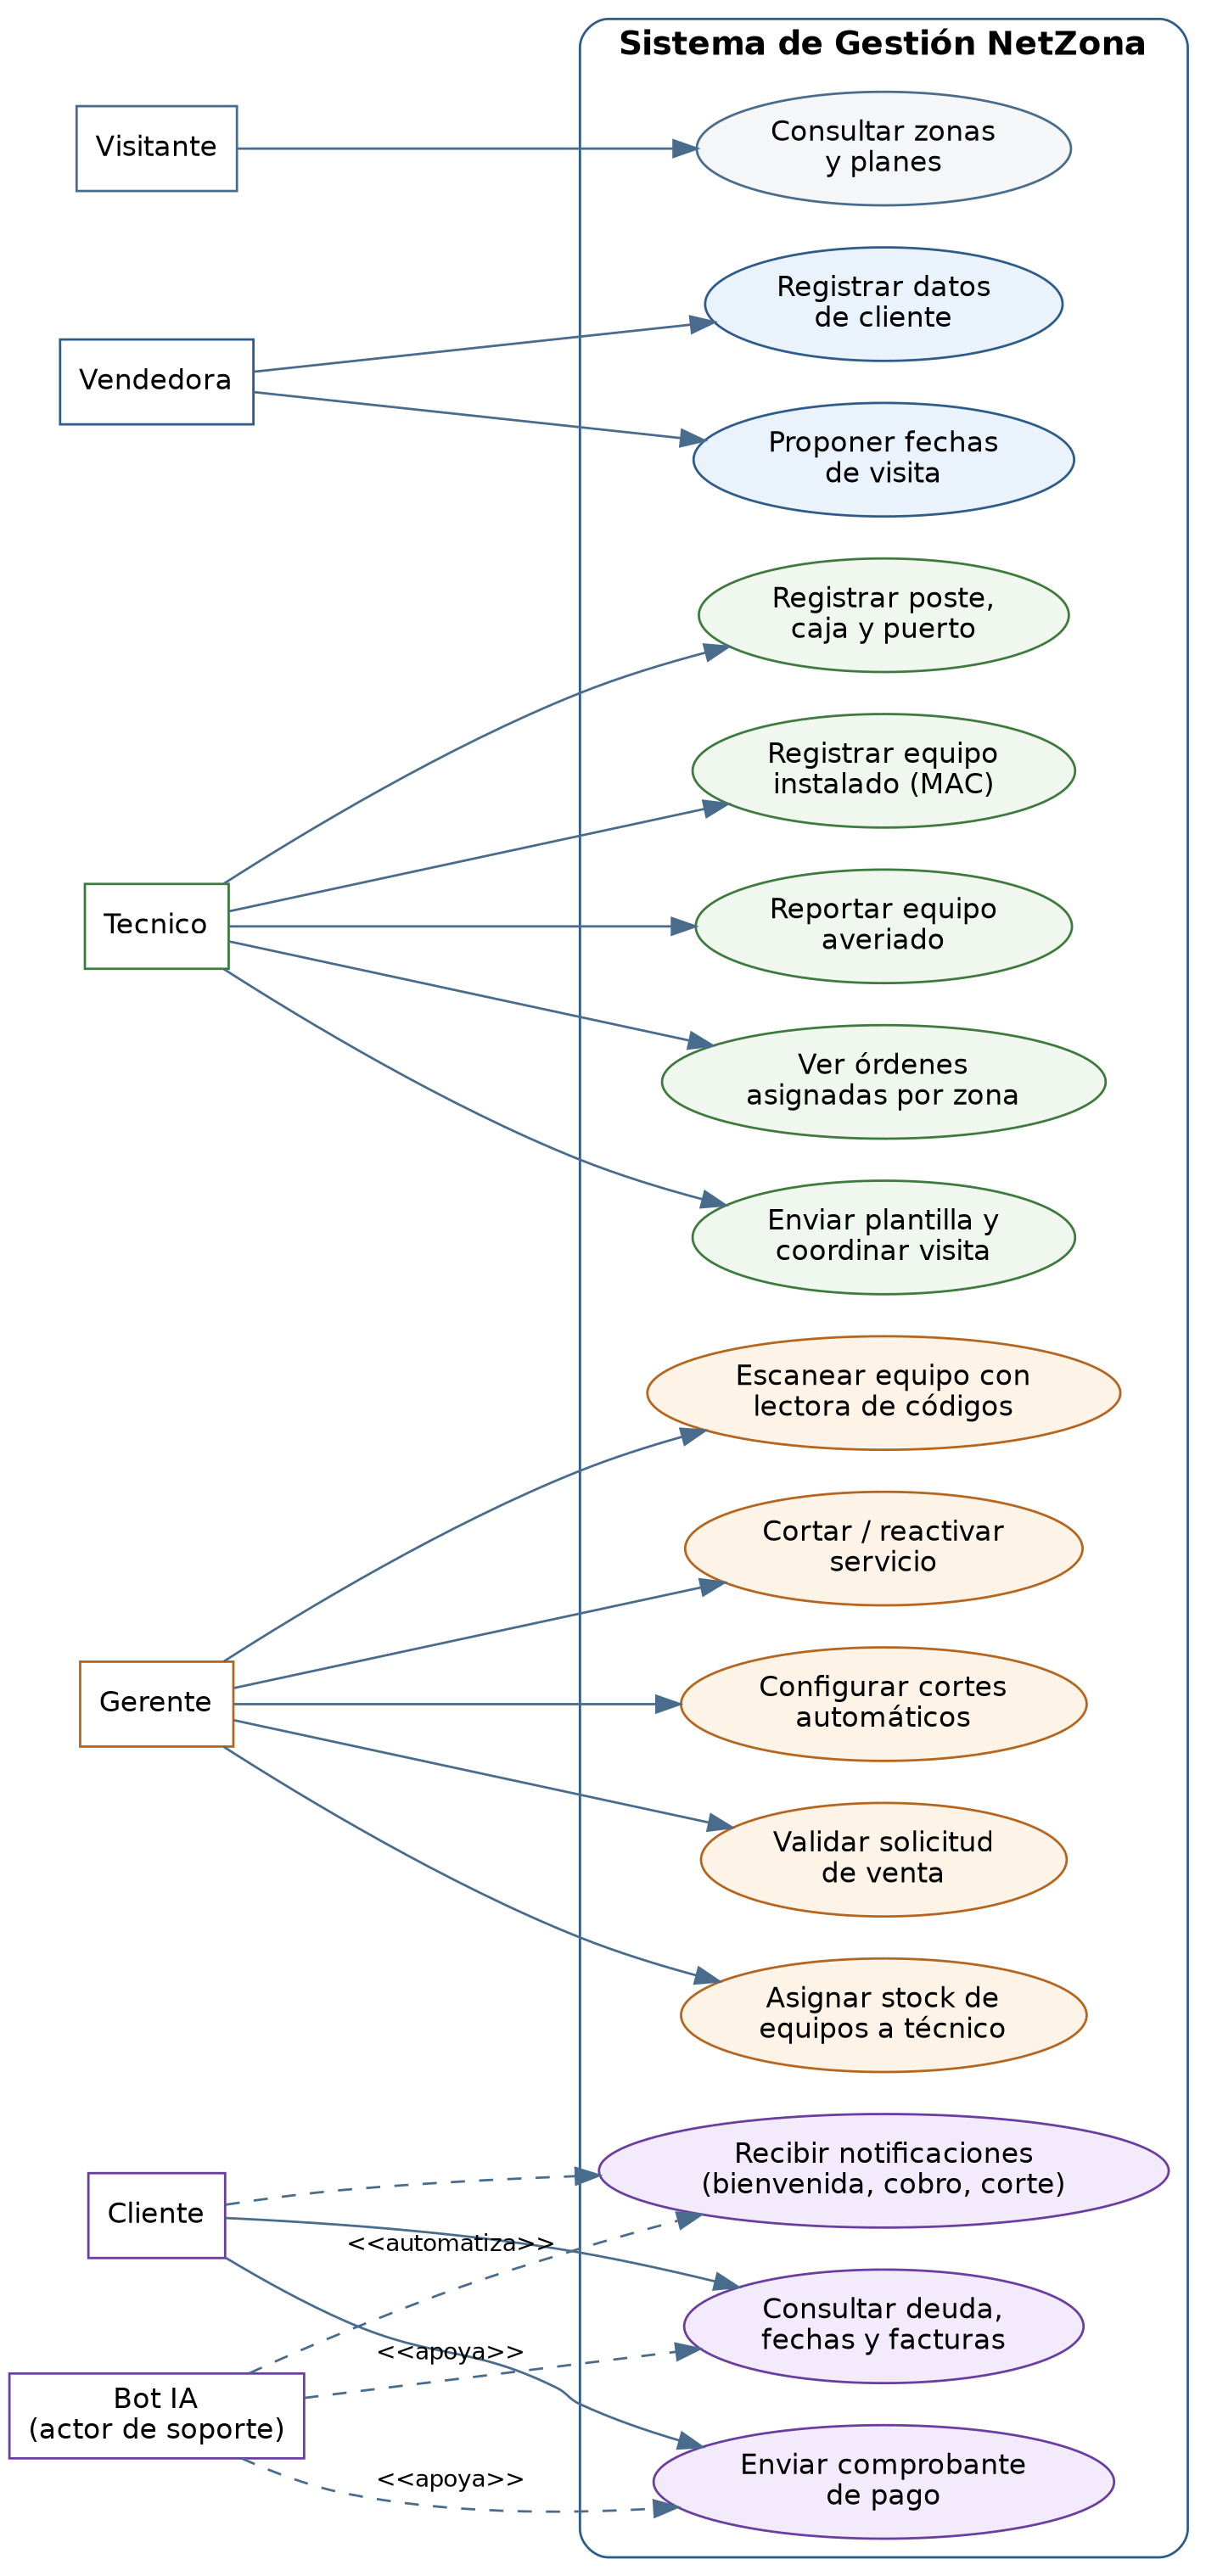
\includegraphics[width=\textwidth,height=0.45\textheight,keepaspectratio]{linea2/casos_uso.png}
\caption{Casos de uso del sistema por actor.}
\label{fig:ce02-casos-uso}
\end{figure}

% ======================================================================
\subsection{Modelo de dominio (diagrama de clases UML)}
\label{sec:ce02-clases}

El diagrama de clases de la \cref{fig:ce02-clases} es el \textbf{modelo de dominio
conceptual} elaborado en la fase de diseño: representa usuarios y roles, el flujo de
clientes y órdenes, la planta externa (postes, cajas NAP y puertos), el inventario de
equipos, los pagos y los mensajes, con sus relaciones y enumeraciones.

\begin{figure}[htbp]
\centering
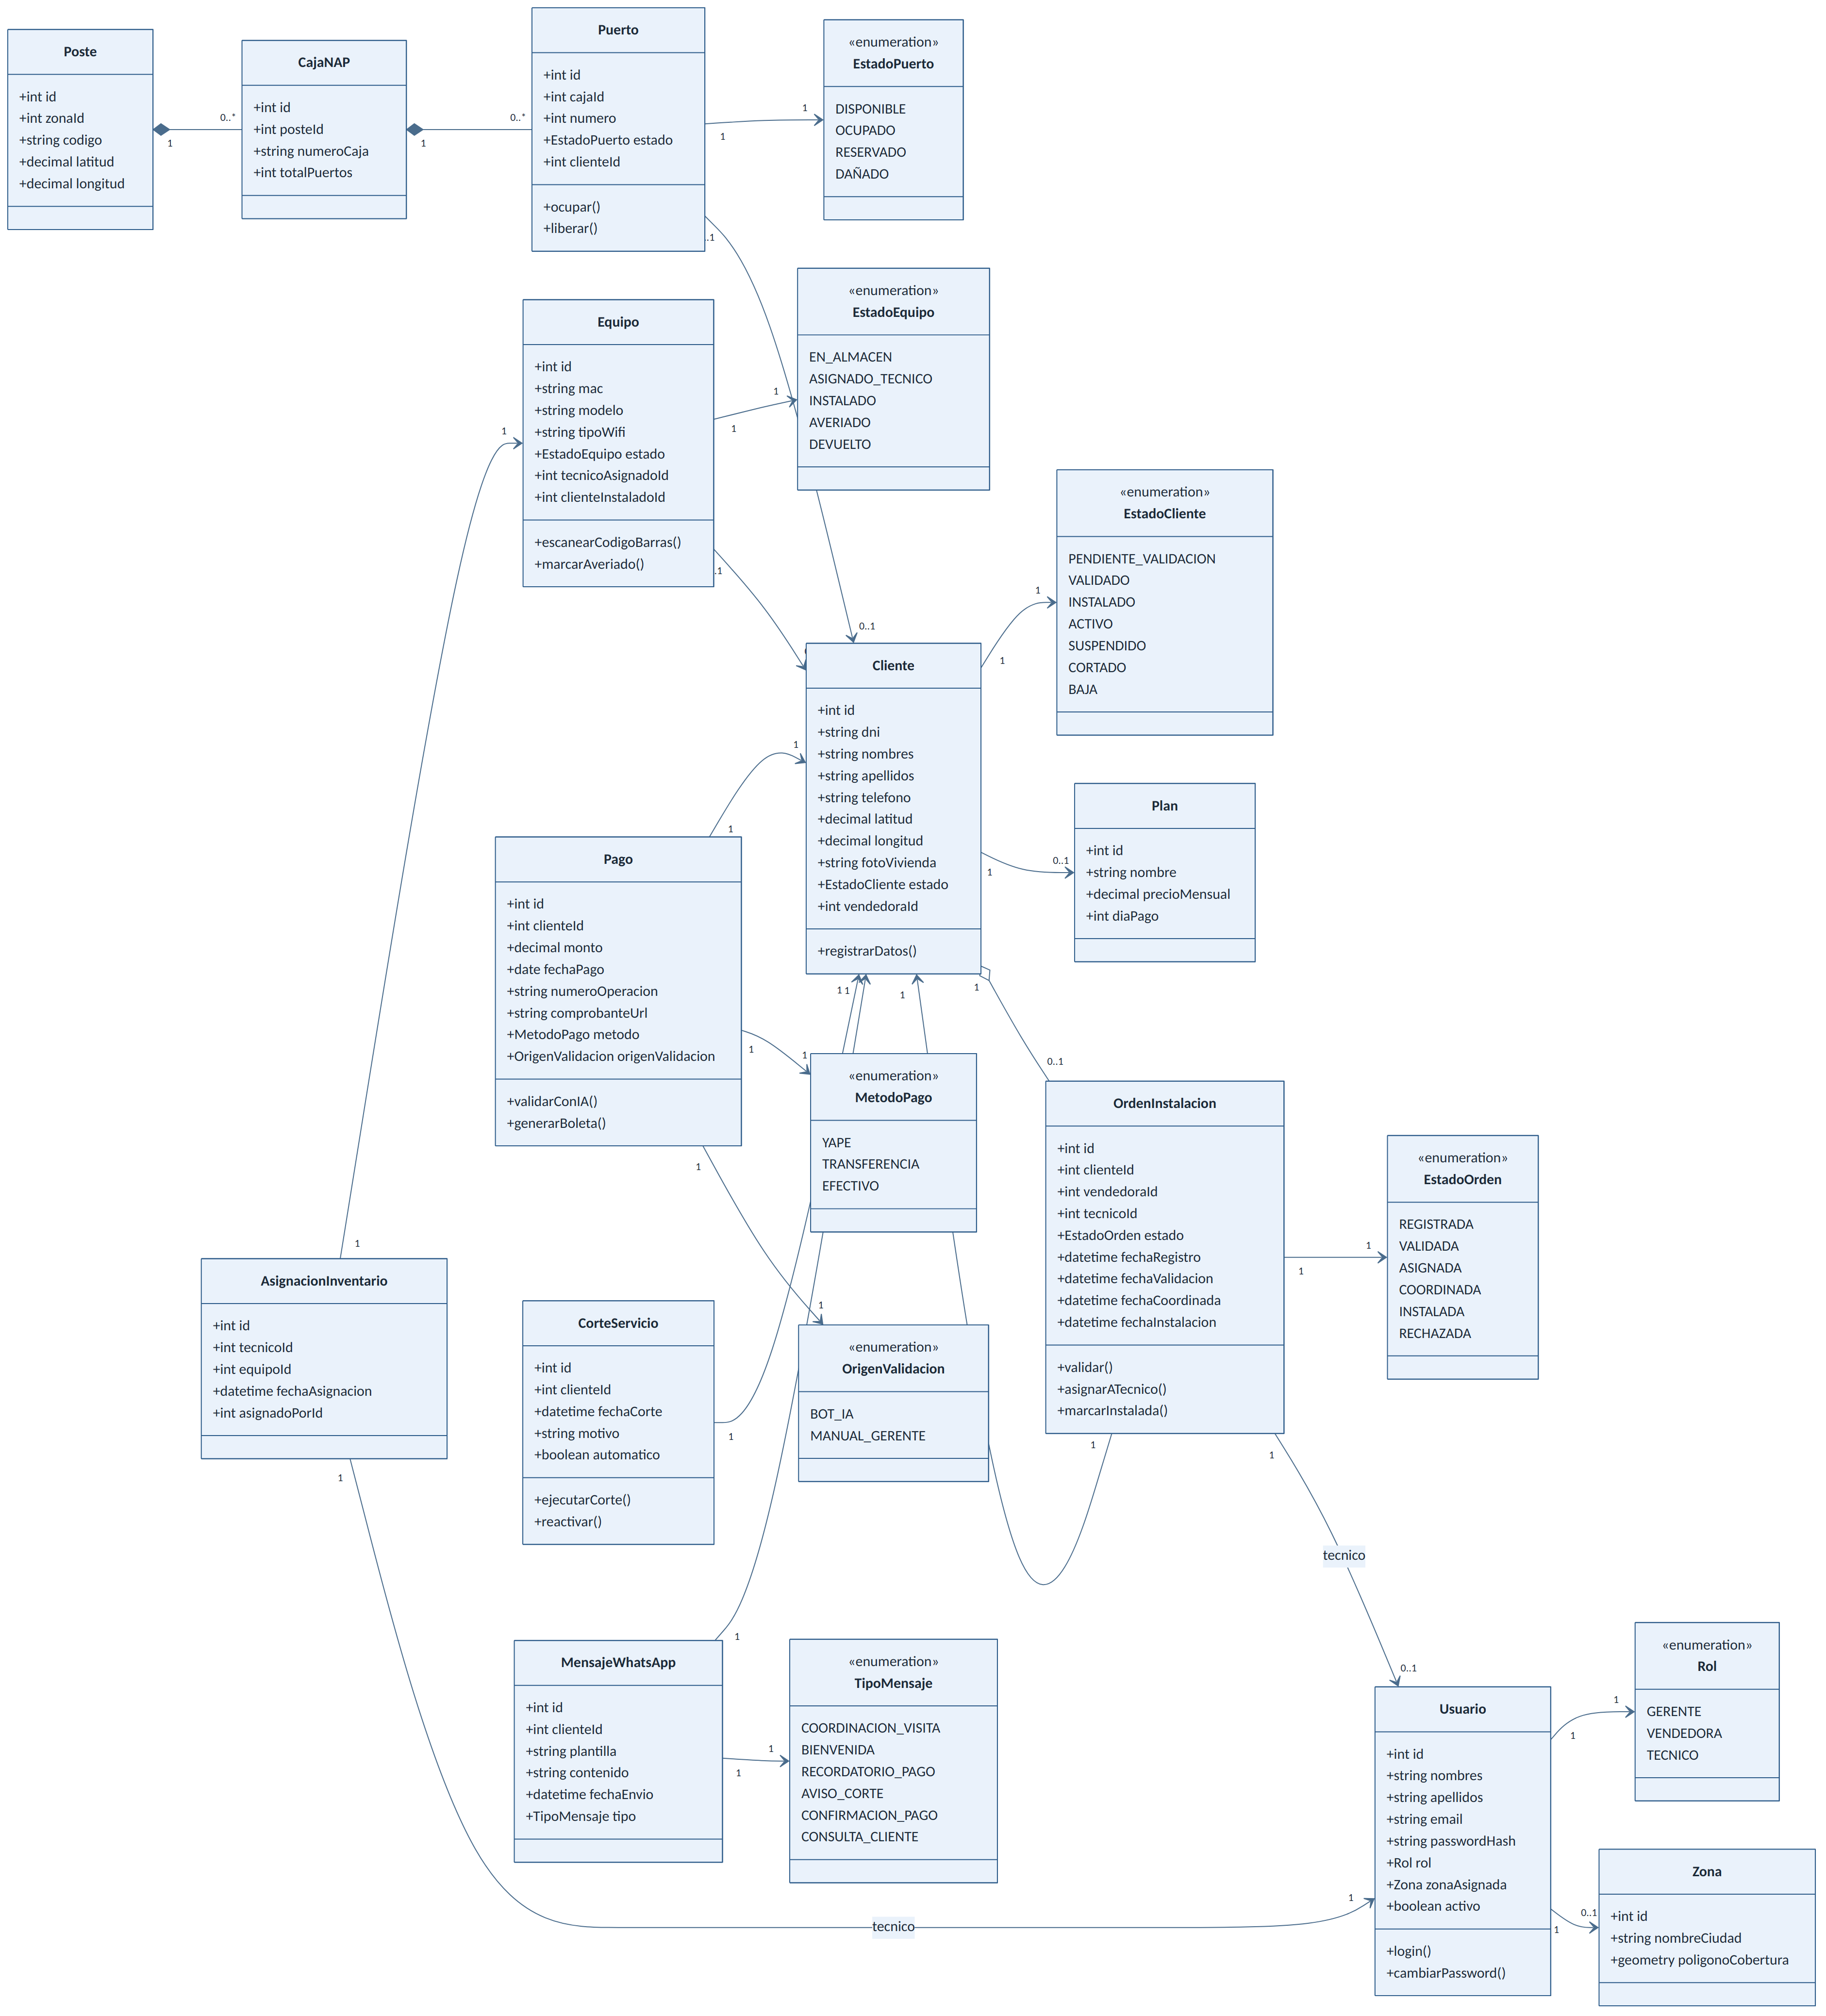
\includegraphics[width=\textwidth,height=0.62\textheight,keepaspectratio]{linea2/clases_dominio.png}
\caption{Modelo de dominio conceptual (diseño).}
\label{fig:ce02-clases}
\end{figure}

Durante la construcción, el modelo se refinó para reflejar el vocabulario real de la
planta de fibra y las necesidades descubiertas en la validación. La
\cref{tab:ce02-mapeo} documenta cada cambio, de modo que el diseño y la base de datos
(\cref{chap:ce02-datos}) sean trazables entre sí.

\begin{table}[htbp]
\centering
\caption{Refinamiento del modelo de dominio: diseño $\rightarrow$ implementación.}
\label{tab:ce02-mapeo}
\small
\begin{tabularx}{\textwidth}{L{3cm}L{3.4cm}X}
\toprule
\textbf{Clase de diseño} & \textbf{Entidad implementada} & \textbf{Motivo del cambio} \\
\midrule
Poste & \texttt{Mufa} + \texttt{Corrida} & En la planta real las cajas cuelgan de una mufa (empalme del troncal) y se unen por corridas de fibra con metraje; el poste no aporta información útil. \\
CajaNAP & \texttt{CajaNap} & Se agrega la mufa de origen y la capacidad de bornes (8 o 16). \\
Puerto & \texttt{Borne} & Término usado por los técnicos; se agregan precinto y potencia óptica (dBm). \\
Equipo & \texttt{Onu} & El equipo instalado es la ONU; se identifica por número de serie único. \\
OrdenInstalacion & Estados de \texttt{Cliente} & La orden no tenía datos propios: su ciclo se modela con los estados del cliente y los campos de aprobación e instalación. \\
CorteServicio & \texttt{Historial} (tipo \texttt{corte}) & Un corte es un evento del cliente; se registra en el historial con usuario y fecha. \\
MensajeWhatsApp & \texttt{MensajeMasivo} + \texttt{MensajeMasivoEnvio} & Se registra cada envío masivo y su resultado por destinatario. \\
AsignacionInventario & \texttt{Onu.tecnico\_id} + fecha & La asignación es un atributo de la ONU. \\
--- & \texttt{Averia}, \texttt{OrdenRetiro}, \texttt{Evidencia} & Operación de campo incorporada en la validación (RF-47, RF-48). \\
--- & \texttt{JornadaVendedor}, \texttt{UbicacionVendedor} & Recorrido del vendedor de campo (RF-49). \\
--- & \texttt{Gasto}, \texttt{ConsultaDocumentoMes} & Gastos por zona (RF-51) y control de cuota de la consulta DNI/RUC. \\
\bottomrule
\end{tabularx}
\end{table}

% ======================================================================
\subsection{Contratos de la API}
\label{sec:ce02-api}

La API está documentada automáticamente con OpenAPI (ruta \texttt{/docs}, oculta en
producción). Todas las rutas, salvo el login y la información pública, exigen un JWT
válido y un rol autorizado.

{\small
\begin{longtable}{L{1.2cm}L{5.2cm}L{2.4cm}L{5.0cm}}
\caption{Endpoints principales del sistema.}\label{tab:ce02-endpoints}\\
\toprule
\textbf{Método} & \textbf{Ruta} & \textbf{Rol} & \textbf{Función} \\
\midrule
\endfirsthead
\toprule
\textbf{Método} & \textbf{Ruta} & \textbf{Rol} & \textbf{Función} \\
\midrule
\endhead
\bottomrule
\endlastfoot
POST & \texttt{/api/auth/login} & Público & Devuelve el JWT (con freno a la fuerza bruta). \\
GET & \texttt{/api/zonas/publicas} & Público & Zonas con cobertura para el sitio web. \\
GET & \texttt{/api/clientes} & Interno & Lista paginada con filtros por zona y estado. \\
POST & \texttt{/api/clientes} & Admin, vendedor & Registra el cliente (estado inicial \texttt{pendiente\_aprobacion}). \\
POST & \texttt{/api/clientes/\{id\}/cortar} & Admin & Aviso por WhatsApp y corte en el MikroTik. \\
POST & \texttt{/api/clientes/\{id\}/reactivar} & Admin & Reactiva y extiende el vencimiento. \\
GET & \texttt{/api/clientes/\{id\}/pppoe-status} & Admin & Sesión PPPoE en tiempo real. \\
POST & \texttt{/api/pagos} & Admin, atención & Registra el pago, emite el recibo y reactiva si corresponde. \\
GET/POST & \texttt{/api/cajas-nap}, \texttt{/api/mufas} & Admin, técnico & Planta externa y bornes. \\
GET/POST & \texttt{/api/onus} & Admin, técnico & Inventario de ONU. \\
GET/POST & \texttt{/api/averias}, \texttt{/api/ordenes-retiro} & Admin, técnico & Operación de campo. \\
GET & \texttt{/api/zonas/\{id\}/wireguard-status} & Admin & Ping, SSH y \emph{handshake} del túnel. \\
POST & \texttt{/api/zonas/\{id\}/wireguard/peer} & Admin & Alta del peer en la VPS. \\
POST & \texttt{/api/zonas/\{id\}/exec} & Admin & Comando RouterOS restringido. \\
POST & \texttt{/api/whatsapp/broadcast-cobros} & Admin & Aviso masivo de cobro. \\
GET & \texttt{/api/cliente/me}, \texttt{/api/cliente/mis-pagos} & Cliente (PIN) & Autoservicio. \\
GET & \texttt{/api/health} & Público & Verificación de salud. \\
\end{longtable}
}

% ======================================================================
\subsection{Diagramas de secuencia}
\label{sec:ce02-secuencias}

Se modelan los cuatro flujos de interacción más importantes. Los diagramas
corresponden al diseño; las notas indican cómo quedó cada paso en la implementación.

\begin{figure}[htbp]
\centering
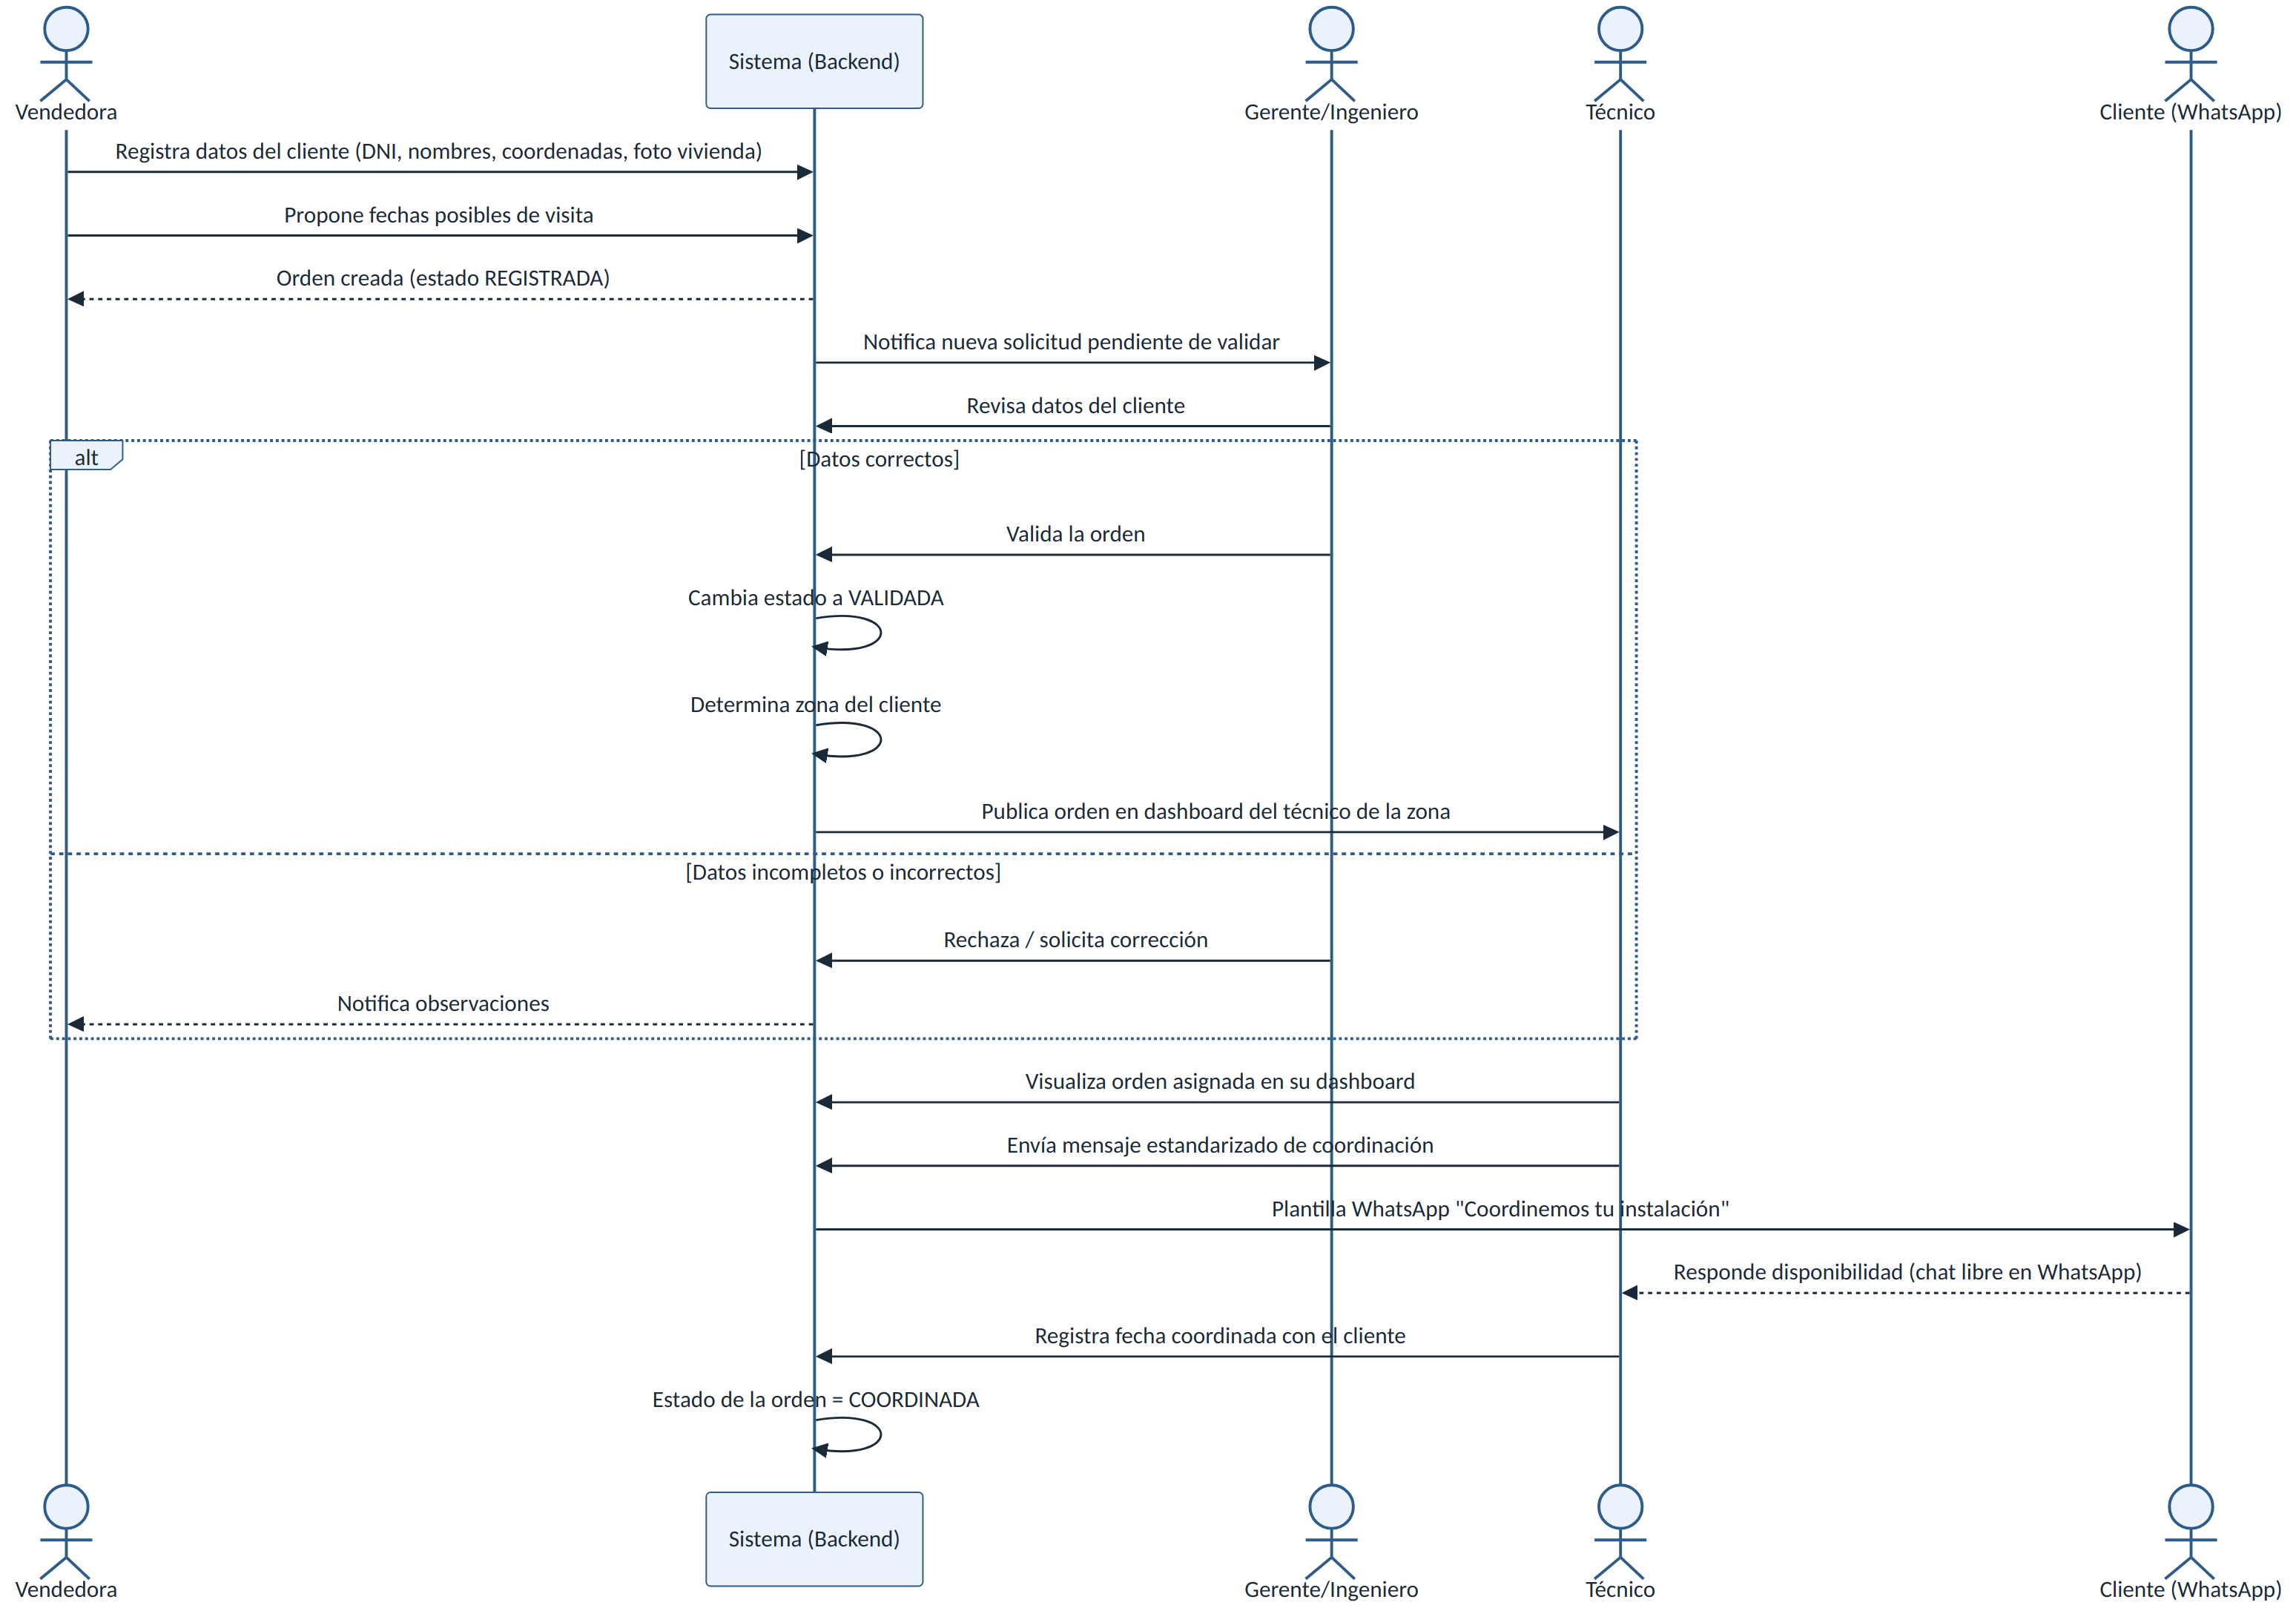
\includegraphics[width=\textwidth,height=0.4\textheight,keepaspectratio]{linea2/seq_venta.png}
\caption{Secuencia: registro de cliente, validación y coordinación de visita.}
\label{fig:ce02-seq-venta}
\end{figure}
\noindent\textit{Implementación:} registro y aprobación completos; el envío de la
plantilla de coordinación y la fecha acordada (RF-13, RF-14) están pendientes.

\begin{figure}[htbp]
\centering
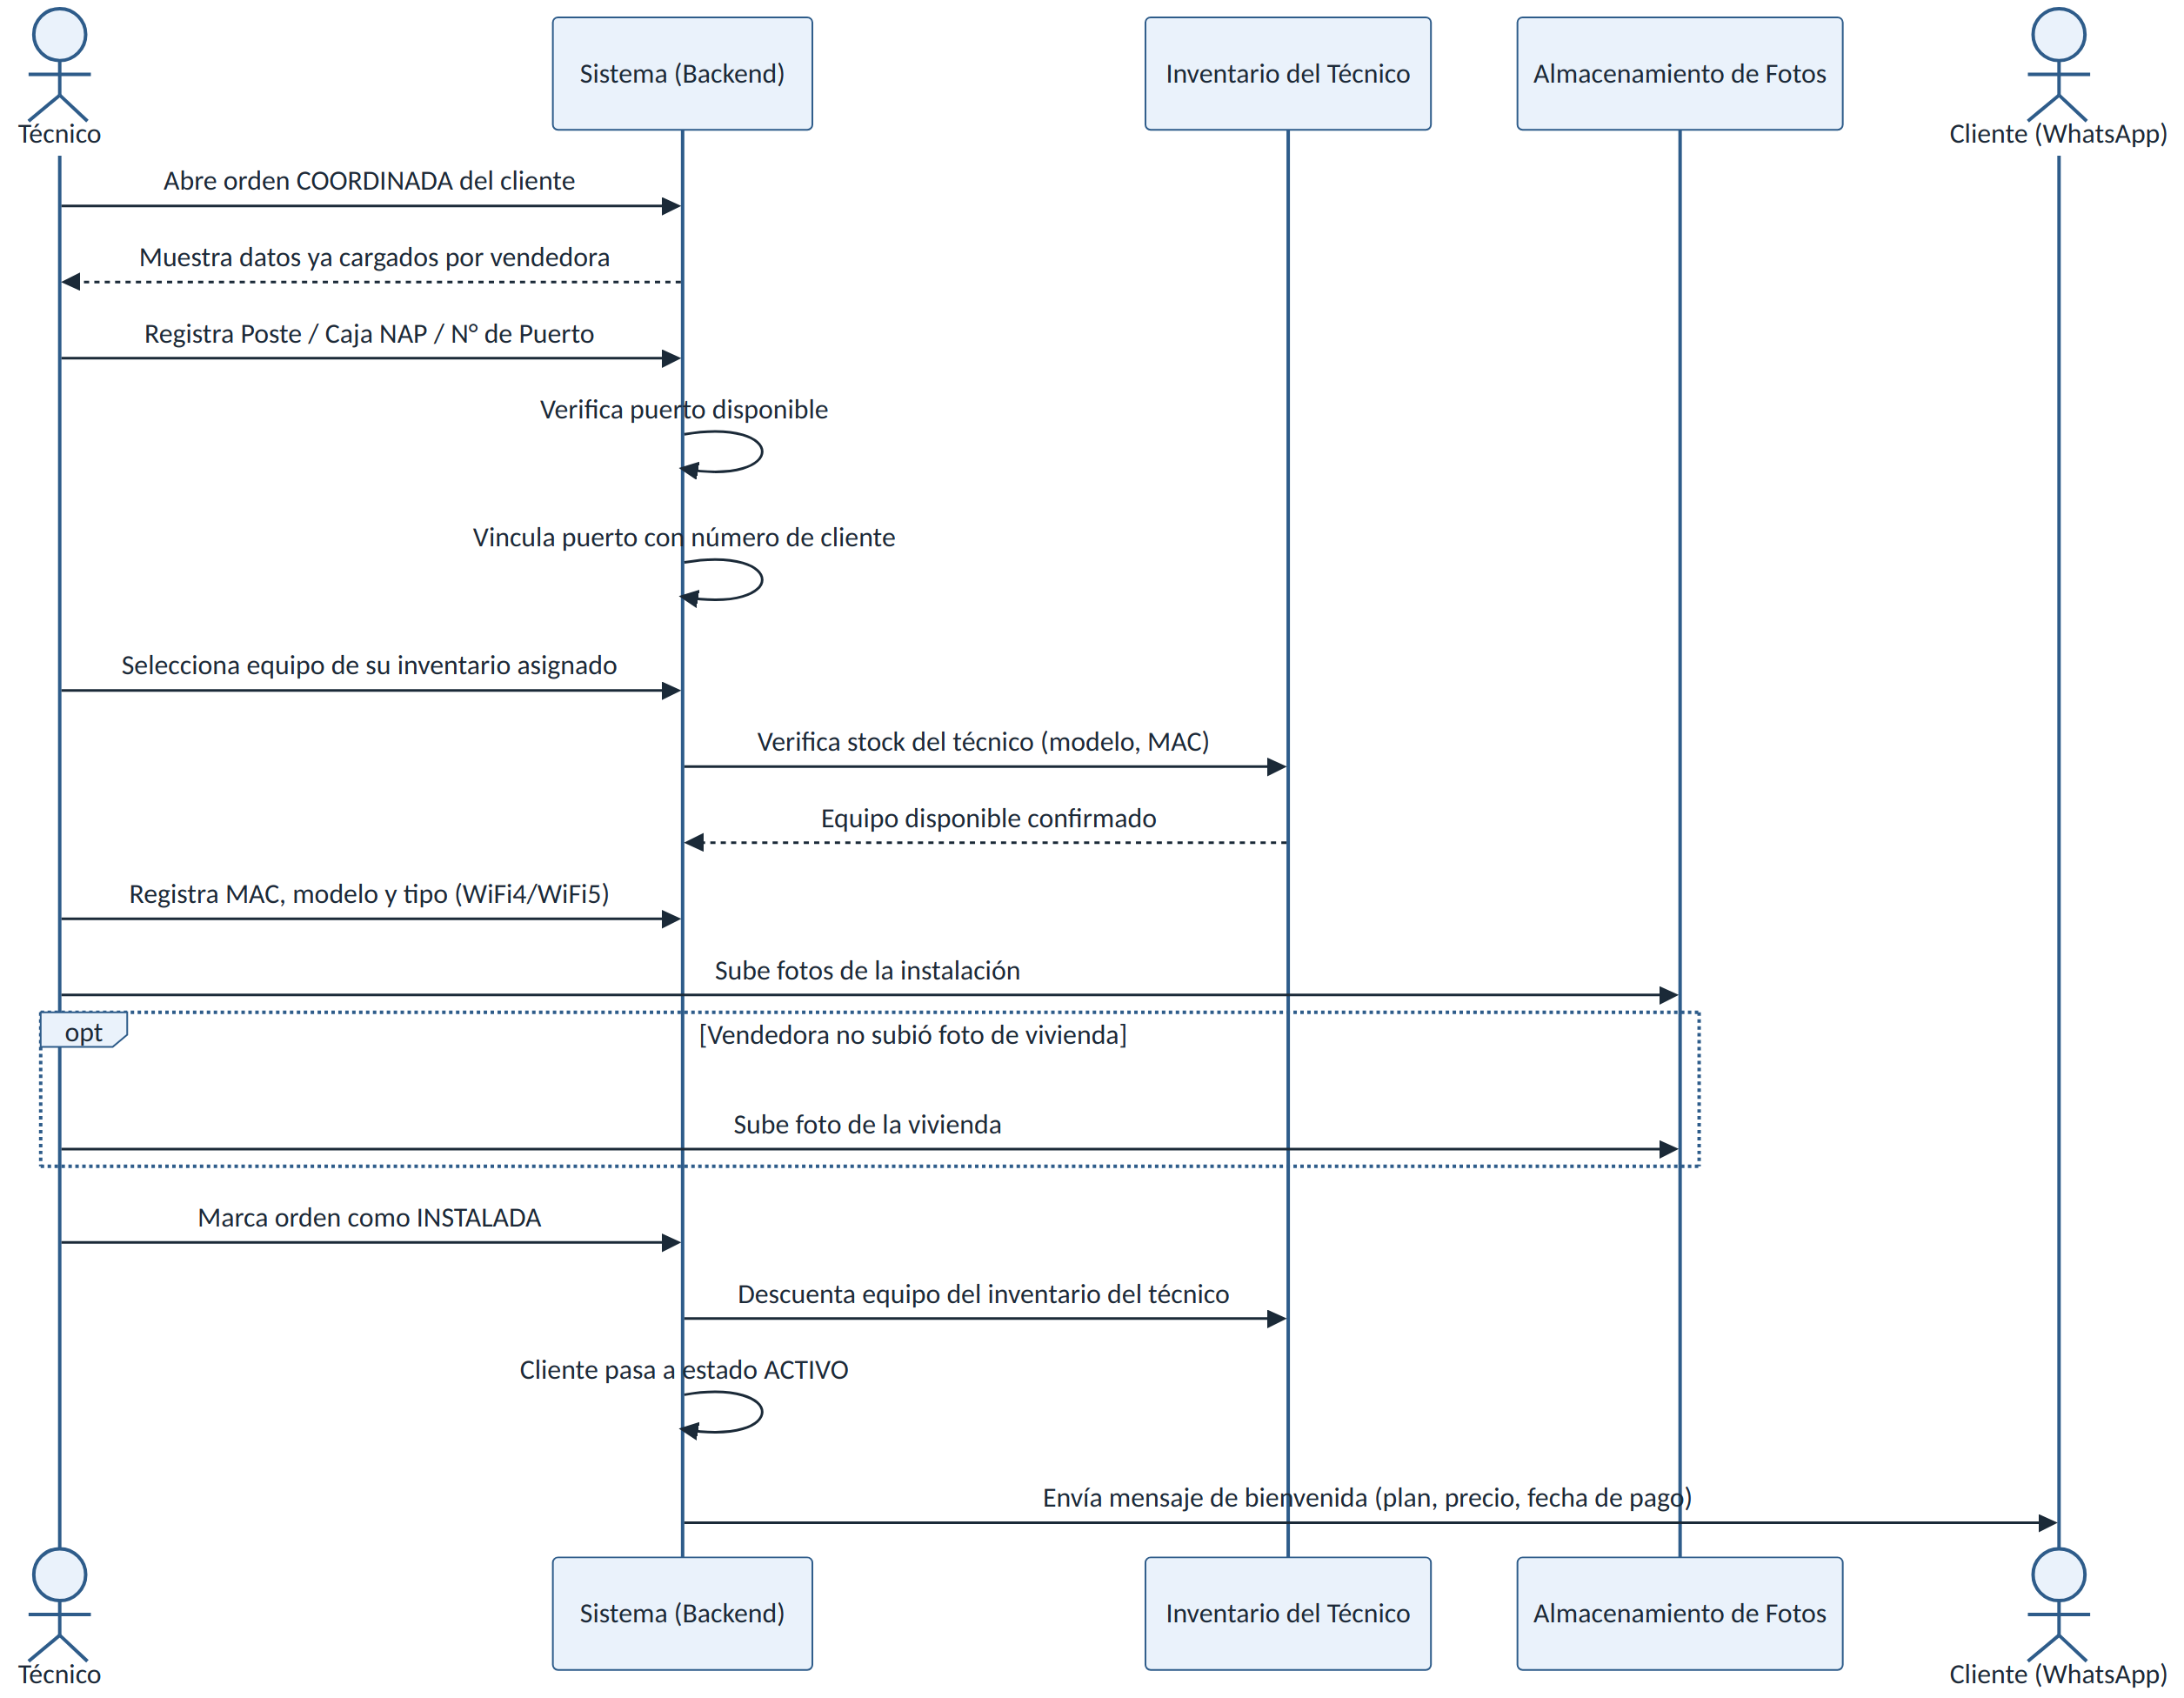
\includegraphics[width=\textwidth,height=0.4\textheight,keepaspectratio]{linea2/seq_instalacion.png}
\caption{Secuencia: registro de caja, borne, equipo y cierre de la instalación.}
\label{fig:ce02-seq-instalacion}
\end{figure}
\noindent\textit{Implementación:} al cerrar, el backend crea el secreto PPPoE en el
MikroTik de la zona por SSH, marca el borne como ocupado y la ONU como instalada, y
activa al cliente.

\begin{figure}[htbp]
\centering
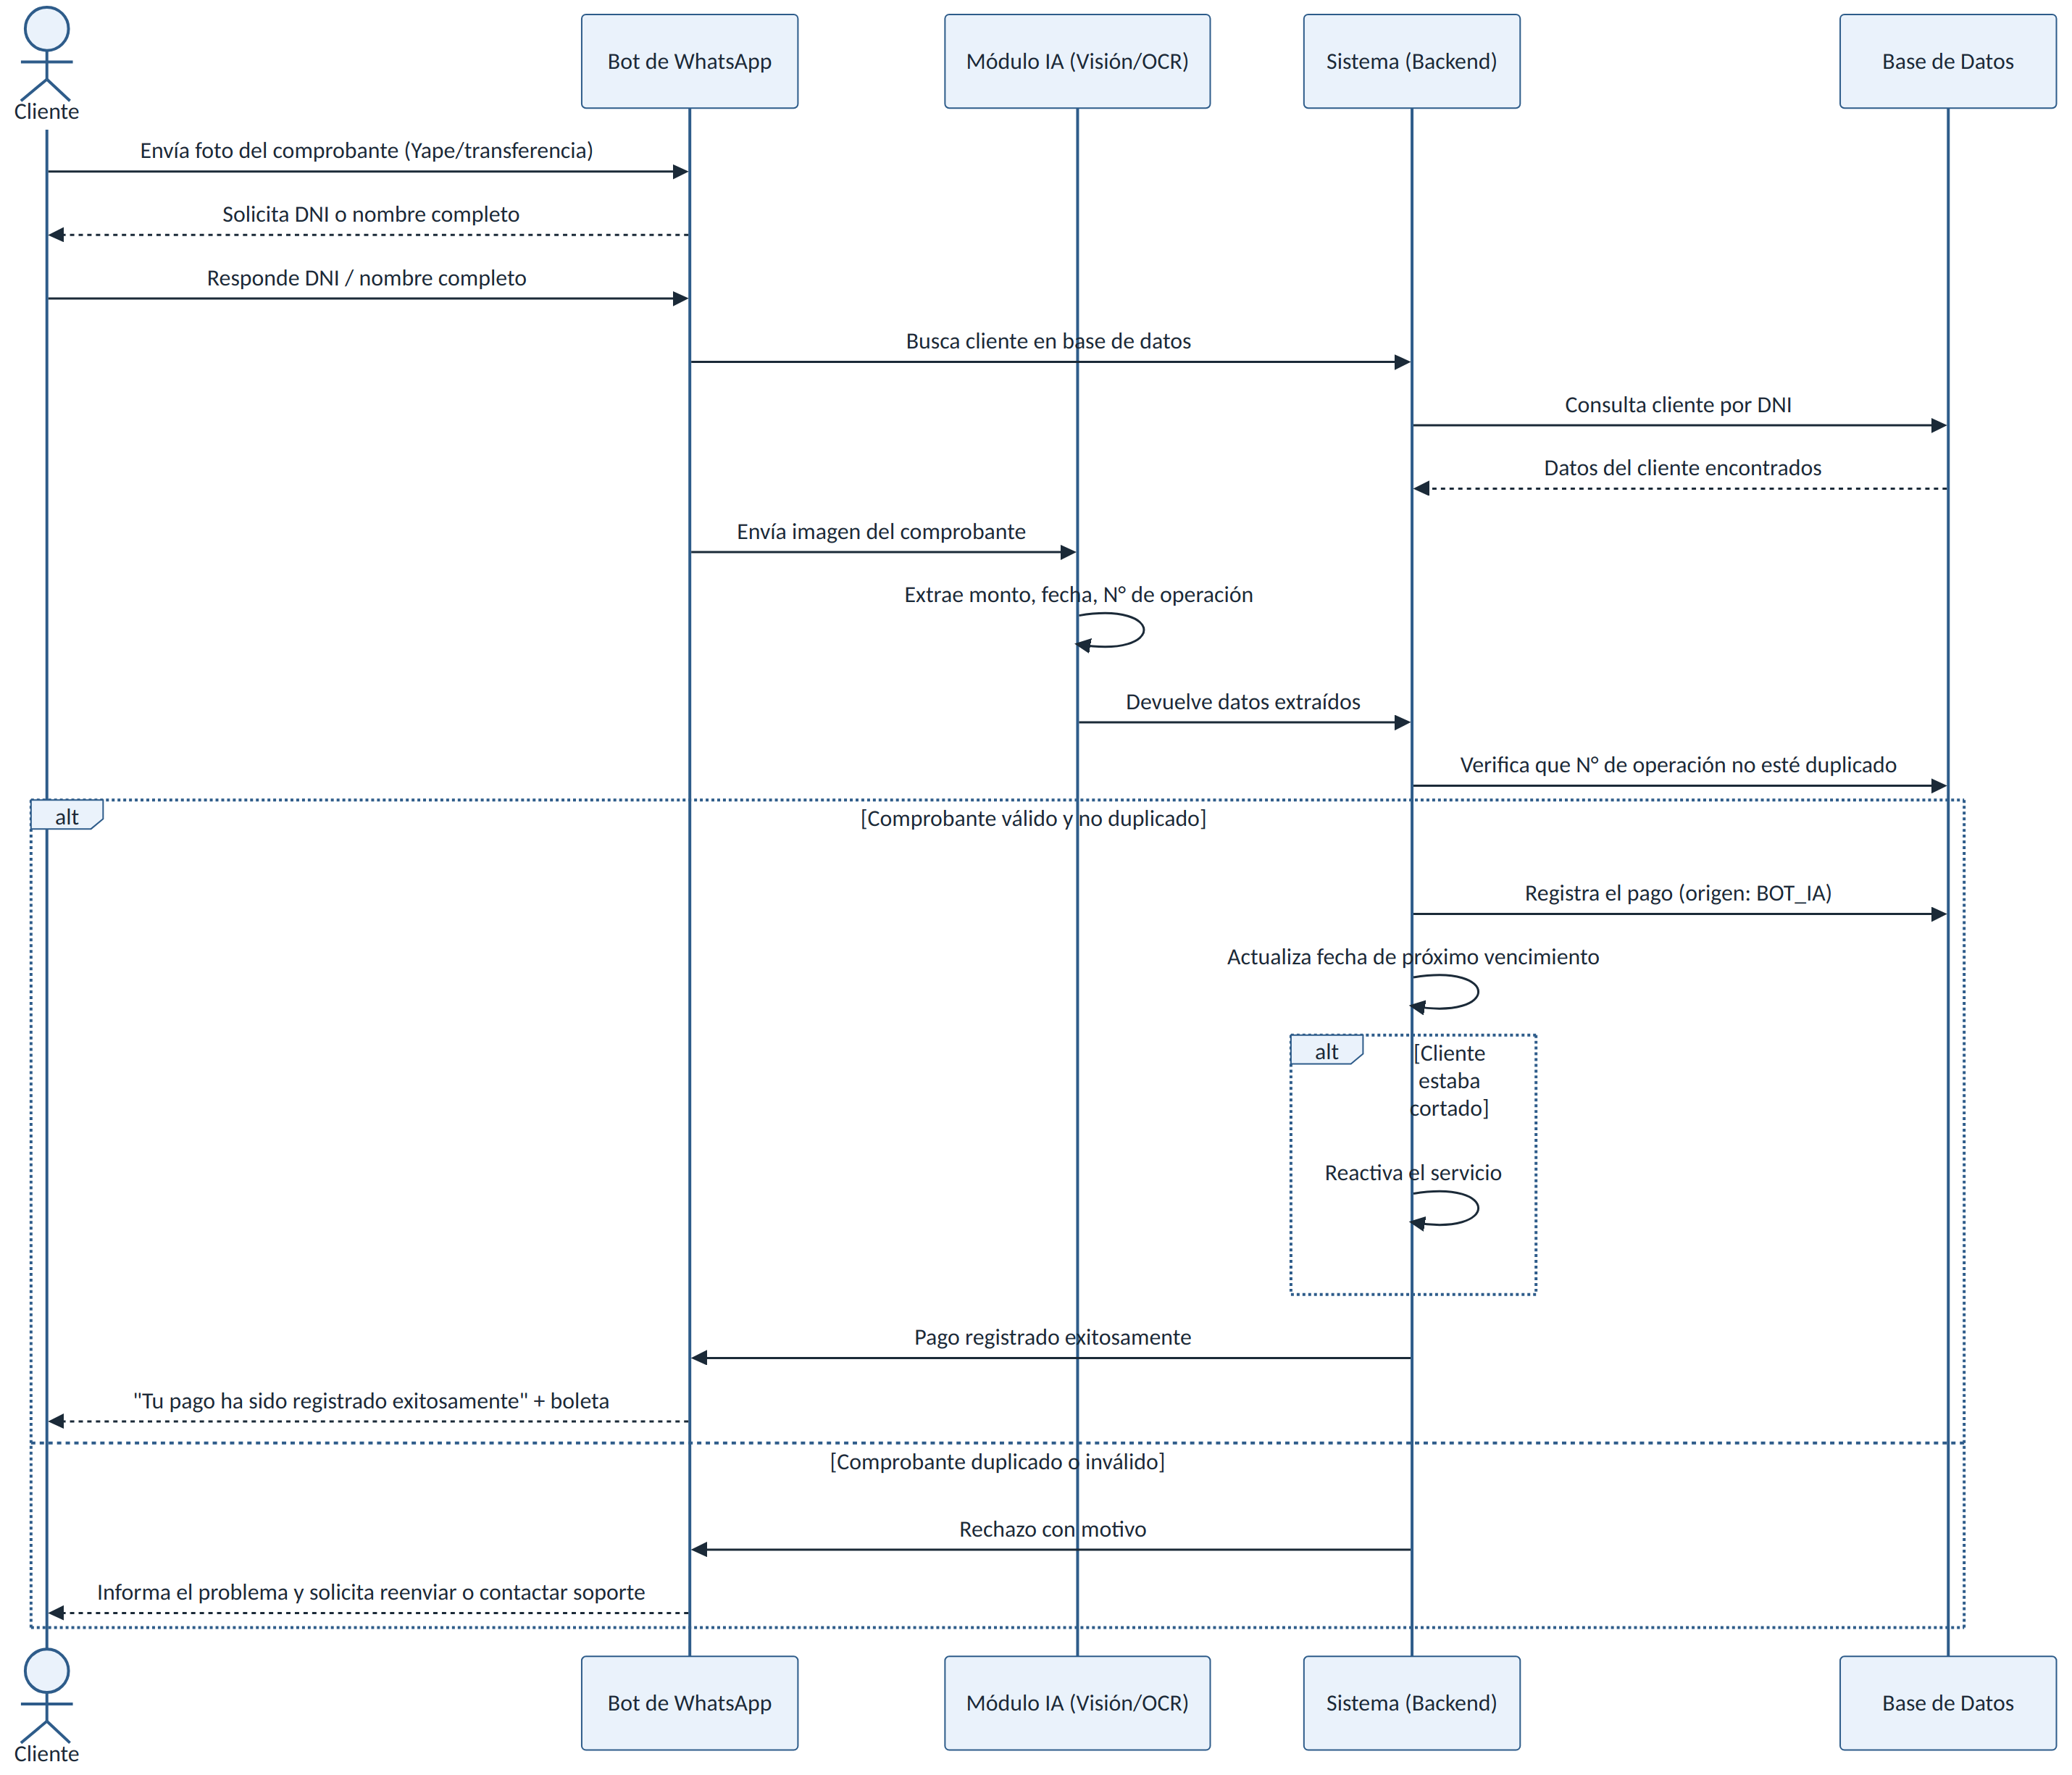
\includegraphics[width=\textwidth,height=0.4\textheight,keepaspectratio]{linea2/seq_pago.png}
\caption{Secuencia (diseño): validación de pago con IA por WhatsApp.}
\label{fig:ce02-seq-pago}
\end{figure}
\noindent\textit{Implementación:} diferida (ADR-06). Hoy el pago lo registra el
personal; la base de datos rechaza números de operación repetidos.

\begin{figure}[htbp]
\centering
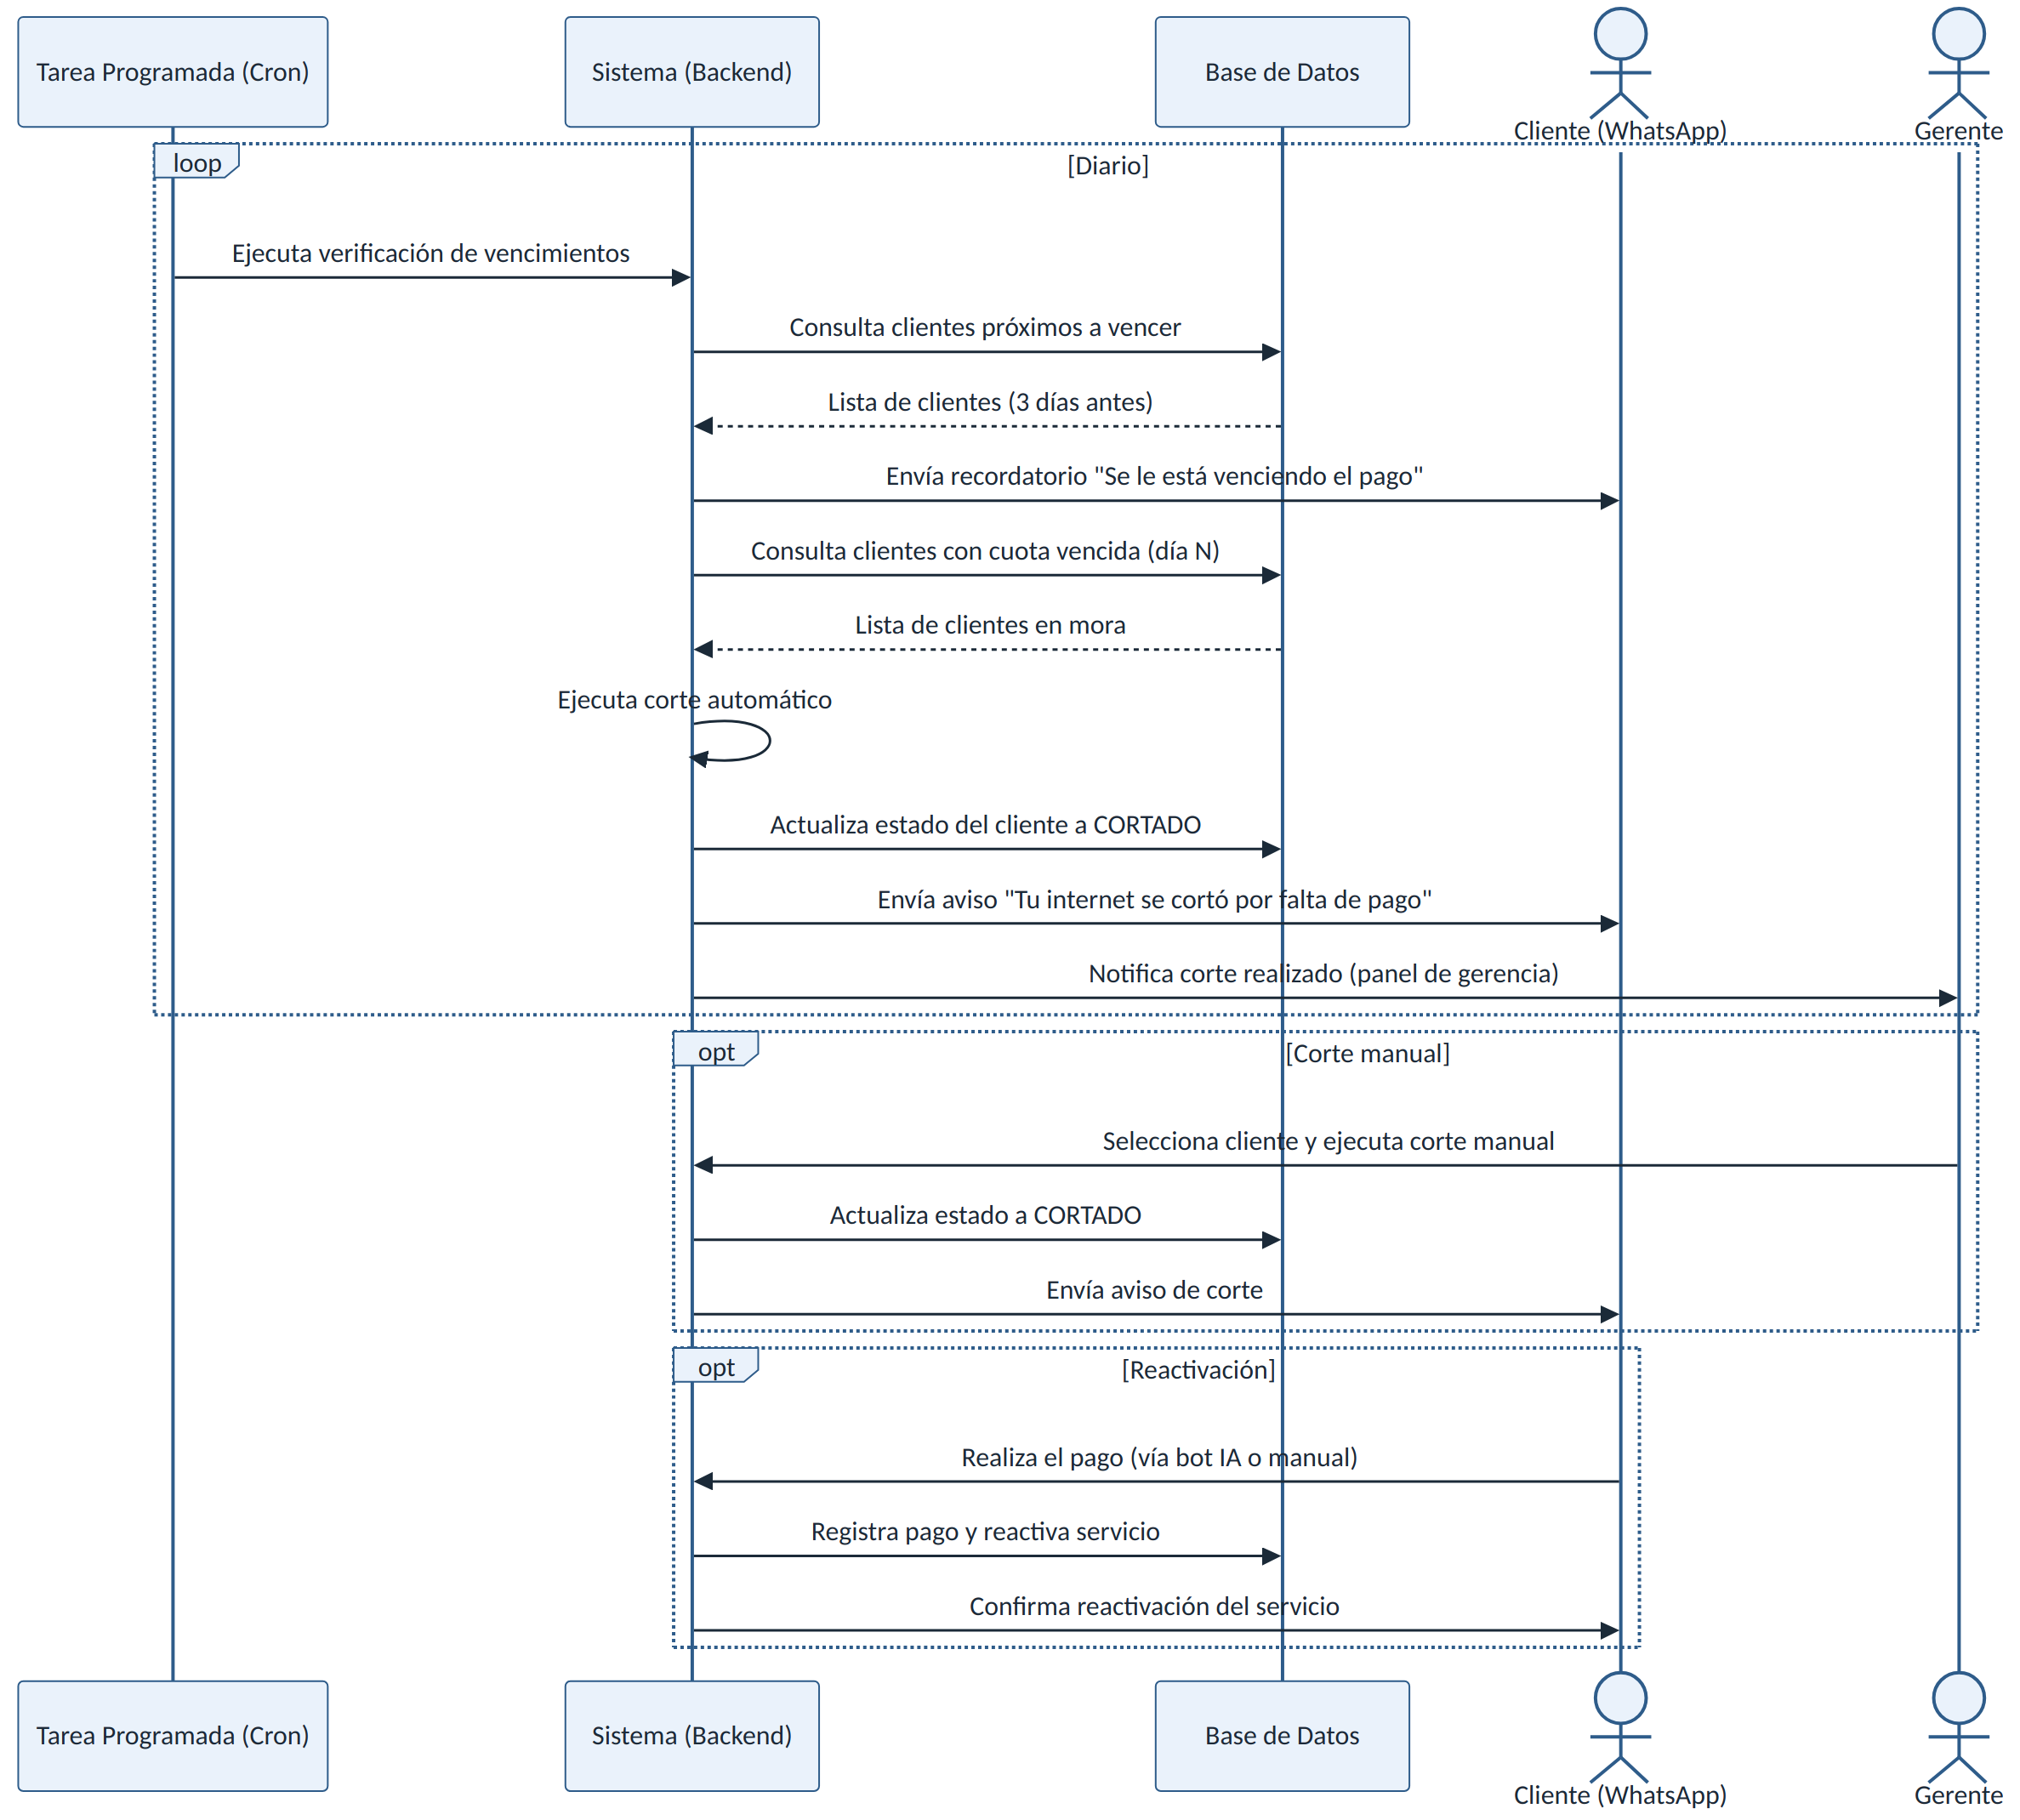
\includegraphics[width=\textwidth,height=0.4\textheight,keepaspectratio]{linea2/seq_corte.png}
\caption{Secuencia: recordatorio, corte automático o manual y reactivación.}
\label{fig:ce02-seq-corte}
\end{figure}
\noindent\textit{Implementación:} el aviso se envía antes del corte (RN-09); el corte
agrega la IP del cliente a la lista de corte configurada para su zona.

% ======================================================================
\subsection{Diagramas de estados}
\label{sec:ce02-estados}

Los diagramas siguientes reflejan los estados reales definidos en
\texttt{backend/app/models.py}.

\tikzset{estado/.style={draw=upeublue,fill=upeublue!8,rounded corners=6pt,font=\scriptsize,
  minimum width=2.3cm,minimum height=7mm,align=center},
  ini/.style={circle,fill=upeublue,minimum size=3mm,inner sep=0pt},
  trans/.style={-{Stealth[length=2mm]},draw=upeublue!80,thick},
  et/.style={font=\tiny,fill=white,inner sep=1pt}}

\begin{figure}[htbp]
\centering
\begin{tikzpicture}[node distance=11mm and 15mm]
  \node[ini] (i) {};
  \node[estado,right=8mm of i] (pend) {pendiente\_aprobacion};
  \node[estado,right=of pend] (apr) {aprobado};
  \node[estado,above=of apr] (rech) {rechazado};
  \node[estado,right=of apr] (act) {activo};
  \node[estado,below=of apr] (noi) {no\_instalado};
  \node[estado,above=of act] (pau) {pausado};
  \node[estado,below=of act] (sus) {suspendido};
  \node[estado,right=14mm of sus] (anu) {anulado};
  \draw[trans] (i) -- (pend);
  \draw[trans] (pend) -- node[et,above]{admin aprueba} (apr);
  \draw[trans] (pend) |- node[et,pos=0.7,above]{admin rechaza} (rech);
  \draw[trans] (apr) -- node[et,above]{instalación cerrada} (act);
  \draw[trans] (apr) -- node[et,left]{no se pudo instalar} (noi);
  \draw[trans] (act.150) -- node[et,left]{pausa} (pau.210);
  \draw[trans] (pau.330) -- node[et,right]{fin de pausa} (act.30);
  \draw[trans] (act.210) -- node[et,left]{corte (mora)} (sus.150);
  \draw[trans] (sus.30) -- node[et,right]{pago / reactivación} (act.330);
  \draw[trans] (sus) -- node[et,below]{baja / retiro} (anu);
  \draw[trans] (act.east) -| node[et,pos=0.3,above]{baja} (anu.north);
\end{tikzpicture}
\caption{Ciclo de vida del cliente (\texttt{EstadoCliente}). Cubre también la antigua
\emph{orden de instalación}.}
\label{fig:ce02-est-cliente}
\end{figure}

\begin{figure}[htbp]
\centering
\begin{tikzpicture}[node distance=9mm and 16mm]
  \node[ini] (i) {};
  \node[estado,right=of i] (alm) {en\_almacen};
  \node[estado,right=of alm] (asg) {asignado\_tecnico};
  \node[estado,right=of asg] (ins) {instalado};
  \node[estado,below=of asg] (dan) {danado};
  \node[estado,above=of asg] (per) {perdido};
  \draw[trans] (i) -- node[et,above]{registro (escaneo)} (alm);
  \draw[trans] (alm) -- node[et,above]{asignar a técnico} (asg);
  \draw[trans] (asg) -- node[et,above]{instalación} (ins);
  \draw[trans] (ins.south) |- node[et,pos=0.25,right]{avería: reemplazo} (dan.east);
  \draw[trans] (asg) -- node[et,right]{reporte de daño} (dan);
  \draw[trans] (asg) -- node[et,right]{extravío} (per);
  \draw[trans] (ins.north) to[out=120,in=60] node[et,above]{retiro en buen estado} (alm.north);
\end{tikzpicture}
\caption{Ciclo de vida de la ONU (\texttt{EstadoOnu}).}
\label{fig:ce02-est-onu}

\vspace{8mm}
\begin{tikzpicture}[node distance=14mm]
  \node[ini] (i) {};
  \node[estado,right=of i] (p) {pendiente};
  \node[estado,right=of p] (a) {asignada};
  \node[estado,right=of a] (e) {en\_proceso};
  \node[estado,right=of e] (r) {resuelta};
  \draw[trans] (i) -- (p);
  \draw[trans] (p) -- node[et,above]{asignar técnico} (a);
  \draw[trans] (a) -- node[et,above]{inicia atención} (e);
  \draw[trans] (e) -- node[et,above]{diagnóstico + fotos} (r);
\end{tikzpicture}
\caption{Ciclo de vida de una avería (\texttt{EstadoAveria}).}
\label{fig:ce02-est-averia}
\end{figure}

El estado de cada borne (\texttt{libre}, \texttt{ocupado}, \texttt{danado}) y de cada
pago (\texttt{pagado}, \texttt{pendiente}, \texttt{vencido}, \texttt{corte\_temporal})
completa el modelo de comportamiento; sus reglas se describen en la
\cref{sec:ce02-rn}.


% ======================================================================
\section{Anexos del entregable}
\label{sec:ce02-e1-anexos}

\begin{table}[H]
\centering
\caption{Anexos exigidos por la plantilla y dónde se encuentran.}
\label{tab:ce02-e1-anexos}
\small
\begin{tabularx}{\textwidth}{L{5cm}XL{2.2cm}}
\toprule
\textbf{Anexo} & \textbf{Ubicación} & \textbf{Estado} \\
\midrule
Acta de validación con stakeholders & \cref{tab:ce02-acta} & Falta fecha y firmas \\
Matriz de trazabilidad de requerimientos & \cref{tab:ce02-trazabilidad} & Completo \\
Diagramas complementarios & Casos de uso (\cref{fig:ce02-casos-uso}), contexto (\cref{fig:ce02-contexto}) y despliegue (\cref{fig:ce02-despliegue}) & Completo \\
Evidencia de sustentación & Exposición breve ante el docente & Por realizar \\
\bottomrule
\end{tabularx}
\end{table}
